\documentclass[12pt,a4paper]{article}
\usepackage[utf8]{inputenc}%Para Tildes y ñ%
\usepackage[spanish]{babel}
\usepackage{amsmath}
\usepackage{amsfonts}
\usepackage{amssymb}
\usepackage{adjustbox}
\usepackage{graphicx} 
\usepackage{pdfpages} %para importar paginas de un pdf 
\usepackage{booktabs}
\usepackage[bookmarks = true, colorlinks=true, linkcolor = black, citecolor = green, menucolor = black, urlcolor = black]{hyperref} 
\usepackage[left=2cm,right=2cm,top=2cm,bottom=2cm]{geometry} 
\usepackage{multirow}
\usepackage{circuitikz}
\usepackage{siunitx}
\usepackage{tabularx}
\usepackage{listings}
\usepackage{verbatimbox}
\usepackage{multicol}
\usepackage{xcolor}
\usepackage{verbatimbox}
\usepackage{float}
\usepackage{textcomp}
\usepackage{caption}
\usepackage{subcaption}
\setcounter{secnumdepth}{0} % ///////////////////////////////////////////// Para que los \section no tenga numeros
\setlength{\tabcolsep}{4pt} % Reduce el espacio horizontal entre columnas
\renewcommand{\arraystretch}{1.2} % Reduce el espacio vertical entre filas

\DeclareRobustCommand{\Colon}{{%
  \ooalign{%
    \hidewidth\raisebox{0.2ex}{/}\kern0.1em\hidewidth\cr
    C\cr
    \hidewidth\kern0.1em\raisebox{0.2ex}{/}\hidewidth\cr
  }%
}}
%Code listing style named "mystyle"
\lstdefinestyle{mystyle}{
  backgroundcolor=\color{backcolour}, commentstyle=\color{codegreen},
  keywordstyle=\color{magenta},
  numberstyle=\tiny\color{codegray},
  stringstyle=\color{codepurple},
  basicstyle=\ttfamily\footnotesize,
  breakatwhitespace=false,         
  breaklines=true,                 
  captionpos=b,                    
  keepspaces=true,                 
  numbers=left,                    
  numbersep=5pt,                  
  showspaces=false,                
  showstringspaces=false,
  showtabs=false,                  
  tabsize=2
}

\input{vspm.hd}

\newcommand{\keywords}[1]{\par\addvspace\baselineskip
\noindent\keywordname\enspace\ignorespaces#1}
\addto\captionsspanish{\renewcommand{\listtablename}{Índice de tablas}}		% Cambiar nombre a lista de tablas   
\addto\captionsspanish{\renewcommand{\tablename}{Tablas}}					% Cambiar nombre a tablas

\usepackage{pdfpages}
\usepackage{enumerate}%listas y viñetas
\author{ Leonardo Serrano Arias C17484  \\Lorena Solís Extteny B97657\\{\small }\\ \\ Profesor: Marco Villalta  \vspace*{3.0in}}
\title{Universidad de Costa Rica\\{\small Facultad de Ingeniería\\Escuela de Ingeniería Eléctrica\\IE0624 – Laboratorio de Microcontroladores\\II ciclo 2024\\\vspace*{0.55in} Proyecto Final }\\ Sistema de Parqueo Inteligente con IoT\vspace*{1.35in}}
\date{27 de Noviembre, 2024} 

\lstset{style=mystyle}
\begin{document} 

\maketitle  
\thispagestyle{empty}%%no numerar la portada
\renewcommand{\thepage}{\roman{page}}
\newpage
\tableofcontents

\listoffigures 

%\listoftables  

%%%%%%%%%%  
\renewcommand{\thepage}{\arabic{page}} 
\setcounter{page}{1}

\newpage
\section{Introducción}
En el contexto actual, la congestión vehicular y la limitada disponibilidad de espacios de estacionamiento en áreas urbanas plantean un desafío significativo para la movilidad y la eficiencia en el uso del tiempo. Los sistemas de parqueo tradicionales suelen requerir supervisión manual, lo que genera demoras y poca transparencia en la gestión de espacios. Ante esta problemática, la implementación de sistemas de parqueo inteligentes se perfila como una solución innovadora y eficiente, aprovechando tecnologías como el Internet de las Cosas (IoT), sensores y plataformas digitales para optimizar el proceso de estacionamiento. Este proyecto busca desarrollar un sistema de parqueo inteligente que automatice la detección de vehículos, la gestión de espacios y la visualización de datos en tiempo real, mejorando la experiencia del usuario y optimizando los recursos disponibles.

El sistema propuesto utiliza un microcontrolador ESP32 como núcleo para coordinar múltiples sensores infrarrojos, servomotores y una pantalla LCD, integrándose con la plataforma móvil Blynk para la monitorización y reserva remota de espacios. Este enfoque permite a los usuarios visualizar la disponibilidad de slots de parqueo en tiempo real tanto en una pantalla local como en sus dispositivos móviles, además de controlar el acceso mediante un mecanismo automatizado de agujas en las entradas y salidas. Con la posibilidad de escalar este sistema y adaptarlo a diferentes entornos, el proyecto no solo contribuye a una mejor gestión de estacionamientos, sino que también sienta las bases para futuras aplicaciones de IoT en el ámbito urbano.

El repositorio utilizado para el desarrollo de este proyecto se encuentra en la siguiente dirección: \url{https://github.com/Leonardo-SA/IE-0624_II_2024_C17484_B97657.git}

\section{Objetivos}

\subsection{Objetivos Generales}
\begin{itemize}
    \item Desarrollar un sistema de parqueo inteligente que permita consultar en tiempo real la disponibilidad de espacios, por medio de una aplicación IoT.
\end{itemize}


\subsection{Objetivos Específicos}
\begin{enumerate}
    \item Implementar un sistema de monitoreo de un parqueo en tiempo real, mediante el uso de un microcontrolador ESP32 y la correcta implementación de un servomotor, así como distintos sensores infrarrojos.
    \item Diseñar una interfaz de usuario para visualizar el estado del estacionamiento y reservar espacios en el mismo.  
    \item Integrar la conectividad WiFi para sincronizar el estado del parqueo con la nube y contar con un sistema de reservas. 
    \item Crear una maqueta del parqueo con agujas automáticas de entrada y salida.
\end{enumerate}


\section{Alcances}
\begin{itemize}
    \item Desarrollar un sistema basado en hardware económico que sea sencilla de implementar y configurar.
    \item Garantizar la comunicación entre los dispositivos y la aplicación IoT. 
    \item Proporcionar una interfaz intuitiva donde se pueda visualizar los espacios del parqueo en un dispositivo con acceso a internet.
\end{itemize}

\section{Justificación}
Un sistema de parqueo inteligente tiene como objetivo solucionar problemas comunes en los estacionamientos tradicionales, como la falta de espacios, el uso ineficiente de los recursos y la pérdida de tiempo en la búsqueda de espacios disponibles. Este tipo de sistemas es especialmente relevante en entornos urbanos y zonas comerciales, donde gestionar eficientemente el espacio es fundamental para optimizar el control interno del parqueo, mejorar la experiencia del usuario y agilizar el proceso de estacionamiento.

En este proyecto se procurará desarrollar este sistema mediante el uso de un ESP32 como microcontrolador central, que ofrece conectividad Wi-Fi integrada, lo cual es clave para implementar el concepto de Internet de las Cosas (IoT). A través de sensores infrarrojos, el sistema podrá detectar la presencia o ausencia de vehículos en cada espacio de estacionamiento, lo cual se mostrará en una pantalla LCD. Además, un servomotor controlará la apertura y cierre de barreras automáticas para regular el acceso a los espacios.

El uso de la plataforma IoT permitirá que el sistema se conecte a una red y proporcione datos en tiempo real sobre la disponibilidad de espacios a los conductores, lo que optimiza el flujo vehicular y reduce la frustración de los usuarios al buscar un lugar para estacionar. Esta información podrá ser accesible desde dispositivos móviles, lo que facilita la toma de decisiones al usuario antes de llegar al estacionamiento.

\section{Marco Teórico}

\subsection{Internet de las Cosas (IoT)}
El término Internet de las cosas (IoT) hace referencia a la red de dispositivos conectados que intercambian datos entre sí y con la nube, gracias a tecnologías avanzadas y al desarrollo de chips de bajo costo. Este concepto permite que objetos cotidianos, como electrodomésticos, vehículos y herramientas, utilicen sensores para recopilar datos y responder de manera inteligente a los usuarios. \cite{iot}

Desde la década de 1990, los avances en miniaturización y eficiencia de los chips han impulsado la incorporación de sensores y procesadores en objetos comunes. Inicialmente, esta integración era limitada debido al tamaño y costo de los dispositivos electrónicos. Con el desarrollo de tecnologías como las etiquetas RFID y chips más pequeños y potentes, la computación se volvió más accesible, permitiendo conectar incluso dispositivos simples, como interruptores de luz, a servicios avanzados de voz. Este ecosistema de dispositivos interconectados, capaces de transmitir y recibir datos automáticamente, constituye el núcleo del Internet de las cosas, transformando hogares, oficinas y empresas con soluciones tecnológicas inteligentes.\cite{iot}

\subsection{ESP-WROOM-32}
El microcontrolador ESP-WROOM-32 es un módulo basado en la familia de chips ESP32 de Espressif System \cite{esp32}. Este módulo es ideal para desarrollar proyectos de IoT debido a su precio accesible, eficiencia energética y avanzadas funcionalidades de conectividad inalámbrica.

Además, este cuenta con una tecnología de 40nm de TSMC, el ESP32 destaca por su rendimiento en términos de consumo energético como de de radiofrecuencia (RF). El diseño del ESP32 incluye componentes como un conmutador de antena, balun RF, amplificador de potencia, amplificador de bajo ruido (LNA), filtros y módulos de gestión de energía. Además, el ESP32 integra circuitos avanzados de calibración que corrigen imperfecciones externas y se adaptan a cambios ambientales, eliminando la necesidad de equipos especializados para pruebas de conectividad Wi-Fi durante la producción masiva.

En términos de conectividad, el ESP32 soporta Wi-Fi en los estándares 802.11 b/g/n, con velocidades de hasta 150 Mbps en la banda de 2.4 GHz, y ofrece características como monitoreo de señales de baliza, fragmentación y reensamblaje de paquetes, así como diversidad de antena. Estas funcionalidades, junto con su capacidad para operar en modos simultáneos (Station, SoftAP y promiscuo), lo convierten en una solución flexible y eficiente para proyectos IoT de última generación. Algunas características principales son: 

\begin{itemize}
    \item \textbf{Procesador:} Doble núcleo con arquitectura de 32 bits, basado en el procesador Tensilica Xtensa, con frecuencia de hasta 240 MHz
    \item \textbf{Memoria:}Cuenta con 520 KB de SRAM y hasta 16 MB de memoria flash.
    \item \textbf{Conectividad:}Soporta tanto Wi-Fi (802.11 b/g/n) como Bluetooth 4.2 (Classic y BLE).
    \item \textbf{I/O:}Dispone de múltiples GPIOs (pines de entrada/salida digital), entradas analógicas, y soporte para interfaces como SPI, I2C, UART, entre otras.
    \item \textbf{Consumo de energía:} Es eficiente en cuanto a consumo, con múltiples modos de ahorro de energía que permiten su uso en aplicaciones alimentadas por batería.
\end{itemize}

A continuación, se muestra la distribución de pines del microcontrolador ESP32. El cual cuenta con 49 pines, 36 pines configurables para I/0, alimentación, ADC/DAC, comunicación y control, como se muestra en la figura \ref{fig:1}.

\begin{figure}[H]
    \centering
    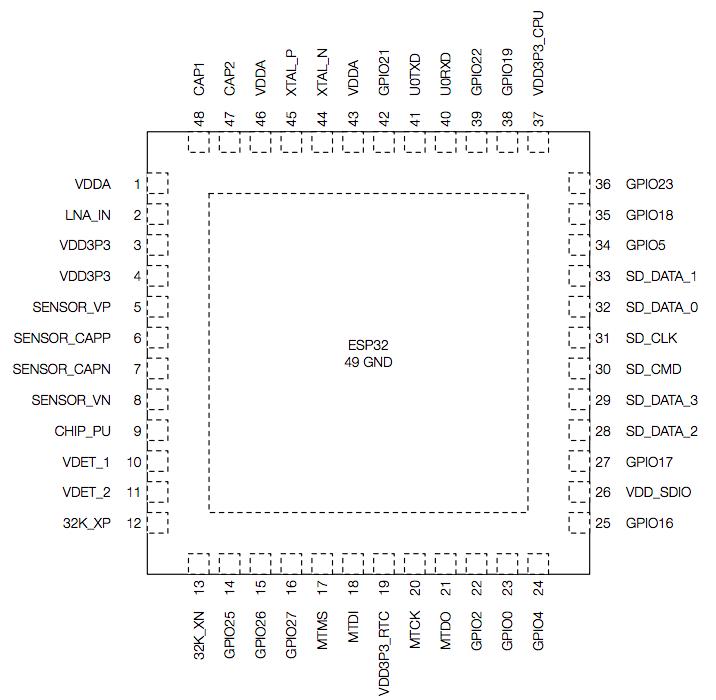
\includegraphics[width=0.5\linewidth]{Imagenes/pines.png}
    \caption{Diagrama de pines ESP32 \cite{esp32}}
    \label{fig:1}
\end{figure}

Seguidamente, se observa en la figura \ref{fig:2} el diagrama de bloques del microcontrolador que muestra toda la arquitectura del mismo.
\begin{figure}[H]
    \centering
    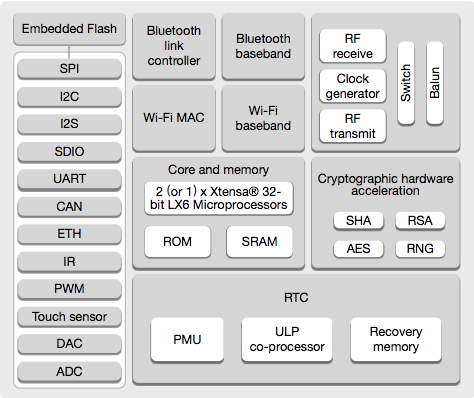
\includegraphics[width=0.5\linewidth]{Imagenes/bd.png}
    \caption{Diagrama de bloques ESP32 \cite{esp32}}
    \label{fig:2}
\end{figure}

Finalmente, se tiene el esquema de potencia del ESP32 que cuenta con tres dominios: VDD3P3\_RTC, VDD3P3\_CPU y VDD\_SDIO. VDD3P3\_RTC alimenta el RTC y el CPU, mientras que VDD3P3\_CPU suministra energía solo al CPU. VDD\_SDIO está conectado a un LDO interno que puede configurarse a 1.8V o al mismo voltaje que VDD3P3\_RTC, y se desactiva automáticamente si comparten la misma conexión. Además, el LDO puede apagarse por software en el modo Deep-sleep para reducir el consumo de energía.

\begin{figure}[H]
    \centering
    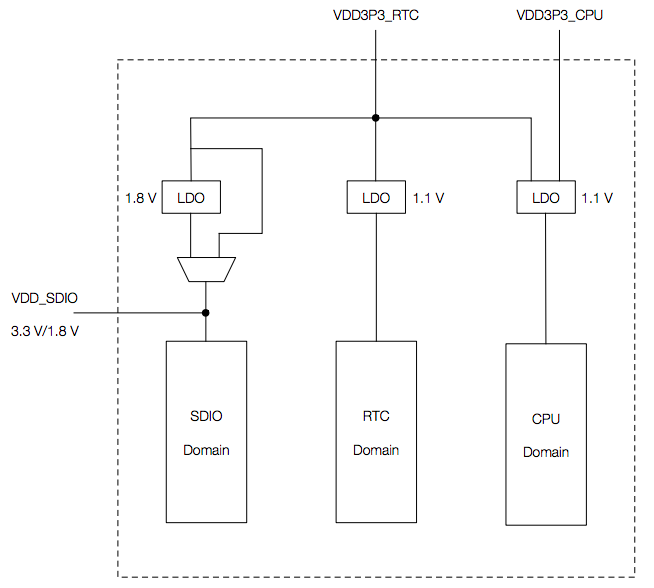
\includegraphics[width=0.5\linewidth]{Imagenes/power.png}
    \caption{Diagrama de potencia ESP32 \cite{esp32}}
    \label{fig:3}
\end{figure}

\subsubsection{Registros y Periféricos}
La tabla que se muestra presenta los registros y periféricos utilizados en el sistema de parqueo inteligente. Detalla los pines del microcontrolador ESP32, los dispositivos conectados, su función dentro del sistema y el modo en que operan (entrada, salida o comunicación). 

\begin{table}[H]
\centering
\caption{Registros y Periféricos del Sistema de Parqueo Inteligente}
\label{tab:registros_perifericos}
\begin{tabularx}{\textwidth}{|c|X|X|X|}
\hline
\textbf{Pin/Registro} & \textbf{Periférico} & \textbf{Uso} & \textbf{Modo de Operación} \\ \hline
25 & Sensor digital infrarrojo & Detección de ocupación en el Slot 1 & Entrada digital \\ \hline
26 & Sensor digital infrarrojo & Detección de ocupación en el Slot 2 & Entrada digital \\ \hline
27 & Sensor digital infrarrojo & Detección de ocupación en el Slot 3 & Entrada digital \\ \hline
32 & Sensor digital infrarrojo & Detección de vehículos entrando al estacionamiento & Entrada digital \\ \hline
33 & Sensor digital infrarrojo & Detección de vehículos saliendo del estacionamiento & Entrada digital \\ \hline
18 & Servomotor & Control de barrera de entrada & Salida PWM \\ \hline
19 & Servomotor & Control de barrera de salida & Salida PWM \\ \hline
34 & Sensor digital infrarrojo & Señalización del estado de la barrera de entrada & Salida digital \\ \hline
35 & Sensor digital infrarrojo & Señalización del estado de la barrera de salida & Salida digital \\ \hline
I2C (0x27) & Pantalla LCD & Visualización de la disponibilidad de espacios & Comunicación I2C \\ \hline
Wi-Fi & Módulo ESP32 & Conexión a la plataforma Blynk & Comunicación inalámbrica \\ \hline
\end{tabularx}
\end{table}

\subsection{Servomotor SG90}
El SG90 \cite{sg90} es un pequeño servomotor ampliamente utilizado en proyectos de electrónica y robótica debido a su bajo costo y facilidad de control. Este servomotor tiene un rango de movimiento angular que típicamente va de 0° a 180°. Algunas de sus características principales son:

\begin{itemize}
    \item \textbf{Torque:}Genera un torque de alrededor de 1.8 kg·cm a 5V.
    \item \textbf{Alimentación:} Funciona con una fuente de 4.8V a 5V.
    \item \textbf{Control:} El servomotor se controla mediante una señal de pulso de ancho variable (PWM) que determina el ángulo de rotación.
    \item \textbf{Velocidad:} 0.1s/60 degree
\end{itemize}

En figura \ref{fig:4} se muestra la funcionalidad de sus pines y un pequeño diagrama:
\begin{figure}[H]
    \centering
    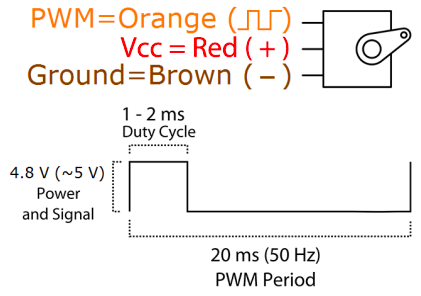
\includegraphics[width=0.5\linewidth]{Imagenes/SG.png}
    \caption{Diagrama del Servomotor SG90 \cite{sg90}}
    \label{fig:4}
\end{figure}

\subsection{Sensor de proximidad infrarojo FC-51}
Este módulo sensor infrarrojo emisor y receptor se puede adaptar a luz ambiente y distancia de detección a través de un potenciómetro que viene incluido en la placa. La distancia de detección está comprendida entre 2 cm y 30 cm, con un ángulo de detección de 35°. Estos infrarrojos emiten señales a cierta frecuencia cuando detectan algún obstáculo (superficie de reflexión). La señal captada por los sensores es acondicionada mediante un circuito comparador, lo que se refleja en un LED indicador de color verde. Dependiendo de la configuración del usuario, se podrán establecer niveles altos (1 lógico) y bajos (0 lógico) de tensión. La señal captada por los sensores puede ser enviada directamente a un circuito de control, como un microcontrolador o una placa Arduino, para ser procesada según las necesidades específicas del usuario o la aplicación. \cite{irsensor}

El sensor requiere un voltaje de funcionamiento que oscila entre 3.3 V y 5 V, y presenta un ángulo de detección de 35°. Los terminales de conexión utilizadas incluyen D0, que corresponde a la señal recibida; GND, que es la tierra; y VCC, para la alimentación. \cite{irsensor}

\begin{figure}[H]
    \centering
    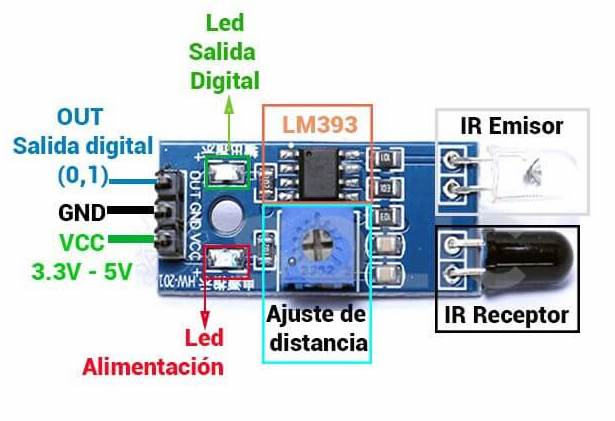
\includegraphics[width=0.5\linewidth]{Imagenes/FC-51.jpeg}
    \caption{Diagrama del sensor de proximidad FC-51\cite{sfc51}}
    \label{fig:5}
\end{figure}

\subsection{I2C 1602 LCD}
El módulo I2C LCD1602 es un dispositivo que permite mostrar texto y caracteres en una pantalla LCD de 16x2 (16 columnas y 2 filas) utilizando el protocolo I2C \cite{lcd}. Este módulo es útil para proyectos basados en Arduino, ya que facilita la visualización de información como lecturas de sensores, mensajes o menús. Integra un chip PCF8574 que convierte los datos seriales del protocolo I2C en datos paralelos compatibles con la pantalla LCD.

El I2C LCD1602 combina un LCD convencional y un módulo I2C montado en la parte posterior de la pantalla. Este módulo I2C expande los puertos de entrada y salida del Arduino mediante el protocolo I2C, que utiliza únicamente dos cables: SDA (datos seriales) y SCL (reloj serial). Esto permite la comunicación simultánea entre varios dispositivos con direcciones únicas, optimizando el uso de recursos.

El módulo I2C convierte las señales del Arduino en comandos para controlar la pantalla LCD. La pantalla está compuesta por 16x2 celdas, cada una formada por una matriz de puntos 5x8 que se encienden o apagan según el voltaje aplicado, permitiendo mostrar diferentes caracteres o símbolos.

La dirección por defecto del módulo es 0x27, aunque en algunos casos puede ser 0x3F. Esta dirección puede modificarse alterando los pines A0, A1 y A2 mediante un puenteado. Por defecto, los pines A0, A1 y A2 están configurados como 1, pero al aplicar un puente, su valor cambia a 0.

El módulo también permite ajustar la retroiluminación y el contraste. La retroiluminación puede habilitarse o deshabilitarse mediante un puente. Además, un potenciómetro ubicado en la parte posterior permite ajustar el contraste, definiendo la claridad del texto mostrado. Girar el potenciómetro en sentido horario incrementa el contraste, mientras que girarlo en sentido antihorario lo reduce.

\subsection{Librerías de Arduino IDE}
\begin{itemize}
    \item \textbf{BlinkSimpleEsp32.h:} Con esta librería permite conectar el modulo ESP32 a la plataforma Blynk. La cual proporciona funciones para conectar el ESP32 a la red, enviar y recibir datos entre el dispositivo y la aplicación Blynk que permite controlar diversos componentes del hardware a través de la interfaz. 
    \item \textbf{Wire.h:}  Esta librería se utiliza para la comunicación I2C, protcolo que permite comunicar   serialmente dos cables que conectan múltiples dispositivos (sensores o pantallas) a un mismo bus. Permite enviar y recibir datos a través de I2C, facilitando la interacción con componentes externos que usan este protocolo.
    \item \textbf{LiquidCrystal\_I2C.h:} Esta librería es específica para controlar pantallas LCD que utilizan el protocolo I2C. Es una forma simplificada de trabajar con pantallas LCD, ya que no necesita manejar múltiples pines para la comunicación, solo dos pines (SCL y SDA) para el I2C. A través de esta librería, se puede escribir texto en una pantalla LCD conectada al ESP3.
    \item \textbf{ESP32Servo.h:} Esta librería proporciona funciones para controlar la posición del servomotor a través de señales PWM (modulación de ancho de pulso), facilitando el control preciso de su movimiento.
    
\end{itemize}


\subsection{Blynk}
Blynk es una plataforma en la nube para IoT (Internet de las Cosas) diseñada para simplificar la creación y gestión de aplicaciones móviles y web personalizables para dispositivos IoT. Su objetivo es ofrecer una solución integral para gestionar todo el ciclo de vida de los dispositivos, desde el prototipo hasta la producción, garantizando seguridad en cada etapa. Blynk permite a los desarrolladores crear aplicaciones móviles de alta calidad, gestionar flotas de dispositivos, realizar pruebas de campo, y desplegar de manera eficiente, todo mientras se facilita la administración de datos, configuraciones, actualizaciones y análisis de rendimiento \cite{blynk}. 

\subsection{Lista de componentes}
Seguidamente, se presenta la lista de componentes necesarios para el desarrollo del parqueo junto con sus costos
\begin{table}[H]
\centering
\begin{tabular}{|c|cc|}
\hline
\textbf{Componente} & \multicolumn{1}{c|}{\textbf{Cantidad}} & \textbf{Precio (\Colon)} \\ \hline
ESP32 & \multicolumn{1}{c|}{1} & 8800 \\ \hline
Protoboard & \multicolumn{1}{c|}{1} & 7832 \\ \hline
Kit de cables & \multicolumn{1}{c|}{1} & 2022 \\ \hline
Servomotores SG90 & \multicolumn{1}{c|}{2} & 4464 \\ \hline
Sensor de proximidad FC-51 & \multicolumn{1}{c|}{5} & 2284 \\ \hline
Cable USB a micro USB & \multicolumn{1}{c|}{1} & 2300 \\ \hline
I2C module & \multicolumn{1}{c|}{1} & 1615 \\ \hline
Pantalla LCD & \multicolumn{1}{c|}{1} & 3900 \\ \hline
Total & \multicolumn{2}{c|}{33217} \\ \hline
\end{tabular}
\caption{Componentes del proyecto con precio}
\label{tab:componentes}
\end{table}

\subsection{Diagrama de flujo del proyecto}
A continuación se muestra el diagrama de flujo del parqueo inteligente que indica el flujo del funcionamiento del mismo:
\begin{figure}[H]
    \centering
    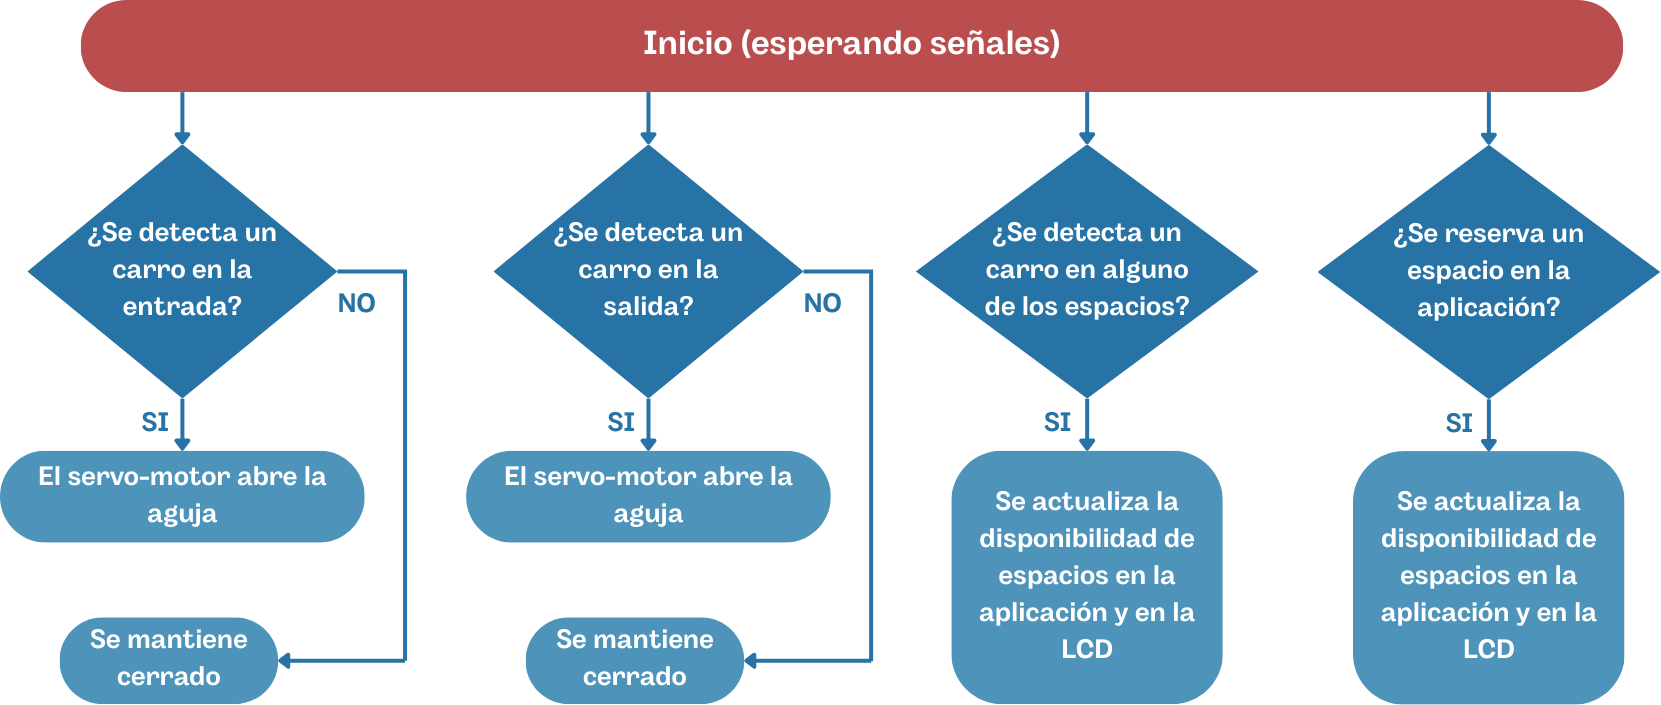
\includegraphics[width=0.9\linewidth]{Imagenes/flow.png}
    \caption{Diagrama de flujo del parqueo inteligente}
    \label{fig:6}
\end{figure}
\subsection{Diagrama de bloques del proyecto}
En la siguiente figura se muestra el diagrama de bloques del parqueo inteligente donde se especifican las señales de entrada y de salida:

\begin{figure}[H]
    \centering
    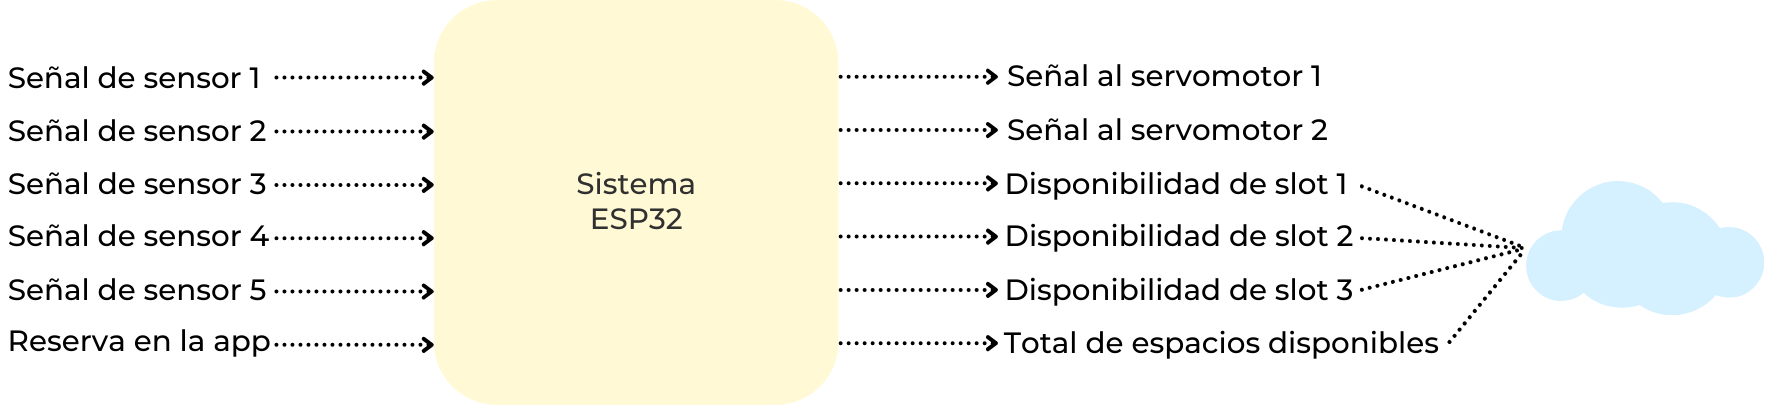
\includegraphics[width=0.85\linewidth]{Imagenes/block.png}
    \caption{Diagrama de bloques del parqueo inteligente}
    \label{fig:7}
\end{figure}
\section{Desarrollo}
En este proyecto se implementó un sistema de parqueo inteligente utilizando un microcontrolador ESP32, sensores infrarrojos, servomotores, una pantalla LCD y la plataforma Blynk para la gestión remota y visualización de datos. Este sistema permite monitorear en tiempo real la disponibilidad de espacios, automatizar el control de las agujas en la entrada y salida, y reservar espacios de parqueo.

\subsection{Componentes y Funcionalidad}
\begin{itemize}
    \item \textbf{Sensores infrarrojos:}
    \begin{itemize}
        \item Tres sensores fueron utilizados para detectar la presencia de vehículos en cada uno de los espacios de parqueo.
        \item Dos sensores adicionales detectaron la entrada o salida de vehículos, activando el servomotor correspondiente para mover la aguja de entrada o salida.
    \end{itemize}

    \item \textbf{Servomotores:}
    \begin{itemize}
        \item Controlan las agujas de entrada y salida, subiendo o bajando en respuesta al estado detectado por los sensores.
    \end{itemize}

    \item \textbf{Pantalla LCD:}
    \begin{itemize}
        \item Muestra en tiempo real el estado de cada espacio de parqueo y el número total de espacios disponibles.
    \end{itemize}

    \item \textbf{Blynk:}
    \begin{itemize}
        \item Permite monitorear la disponibilidad de los espacios a través de una aplicación móvil.
        \item Incluye un switch para reservar espacios de forma remota.
    \end{itemize}
\end{itemize}

\begin{figure}[H]
    \centering
    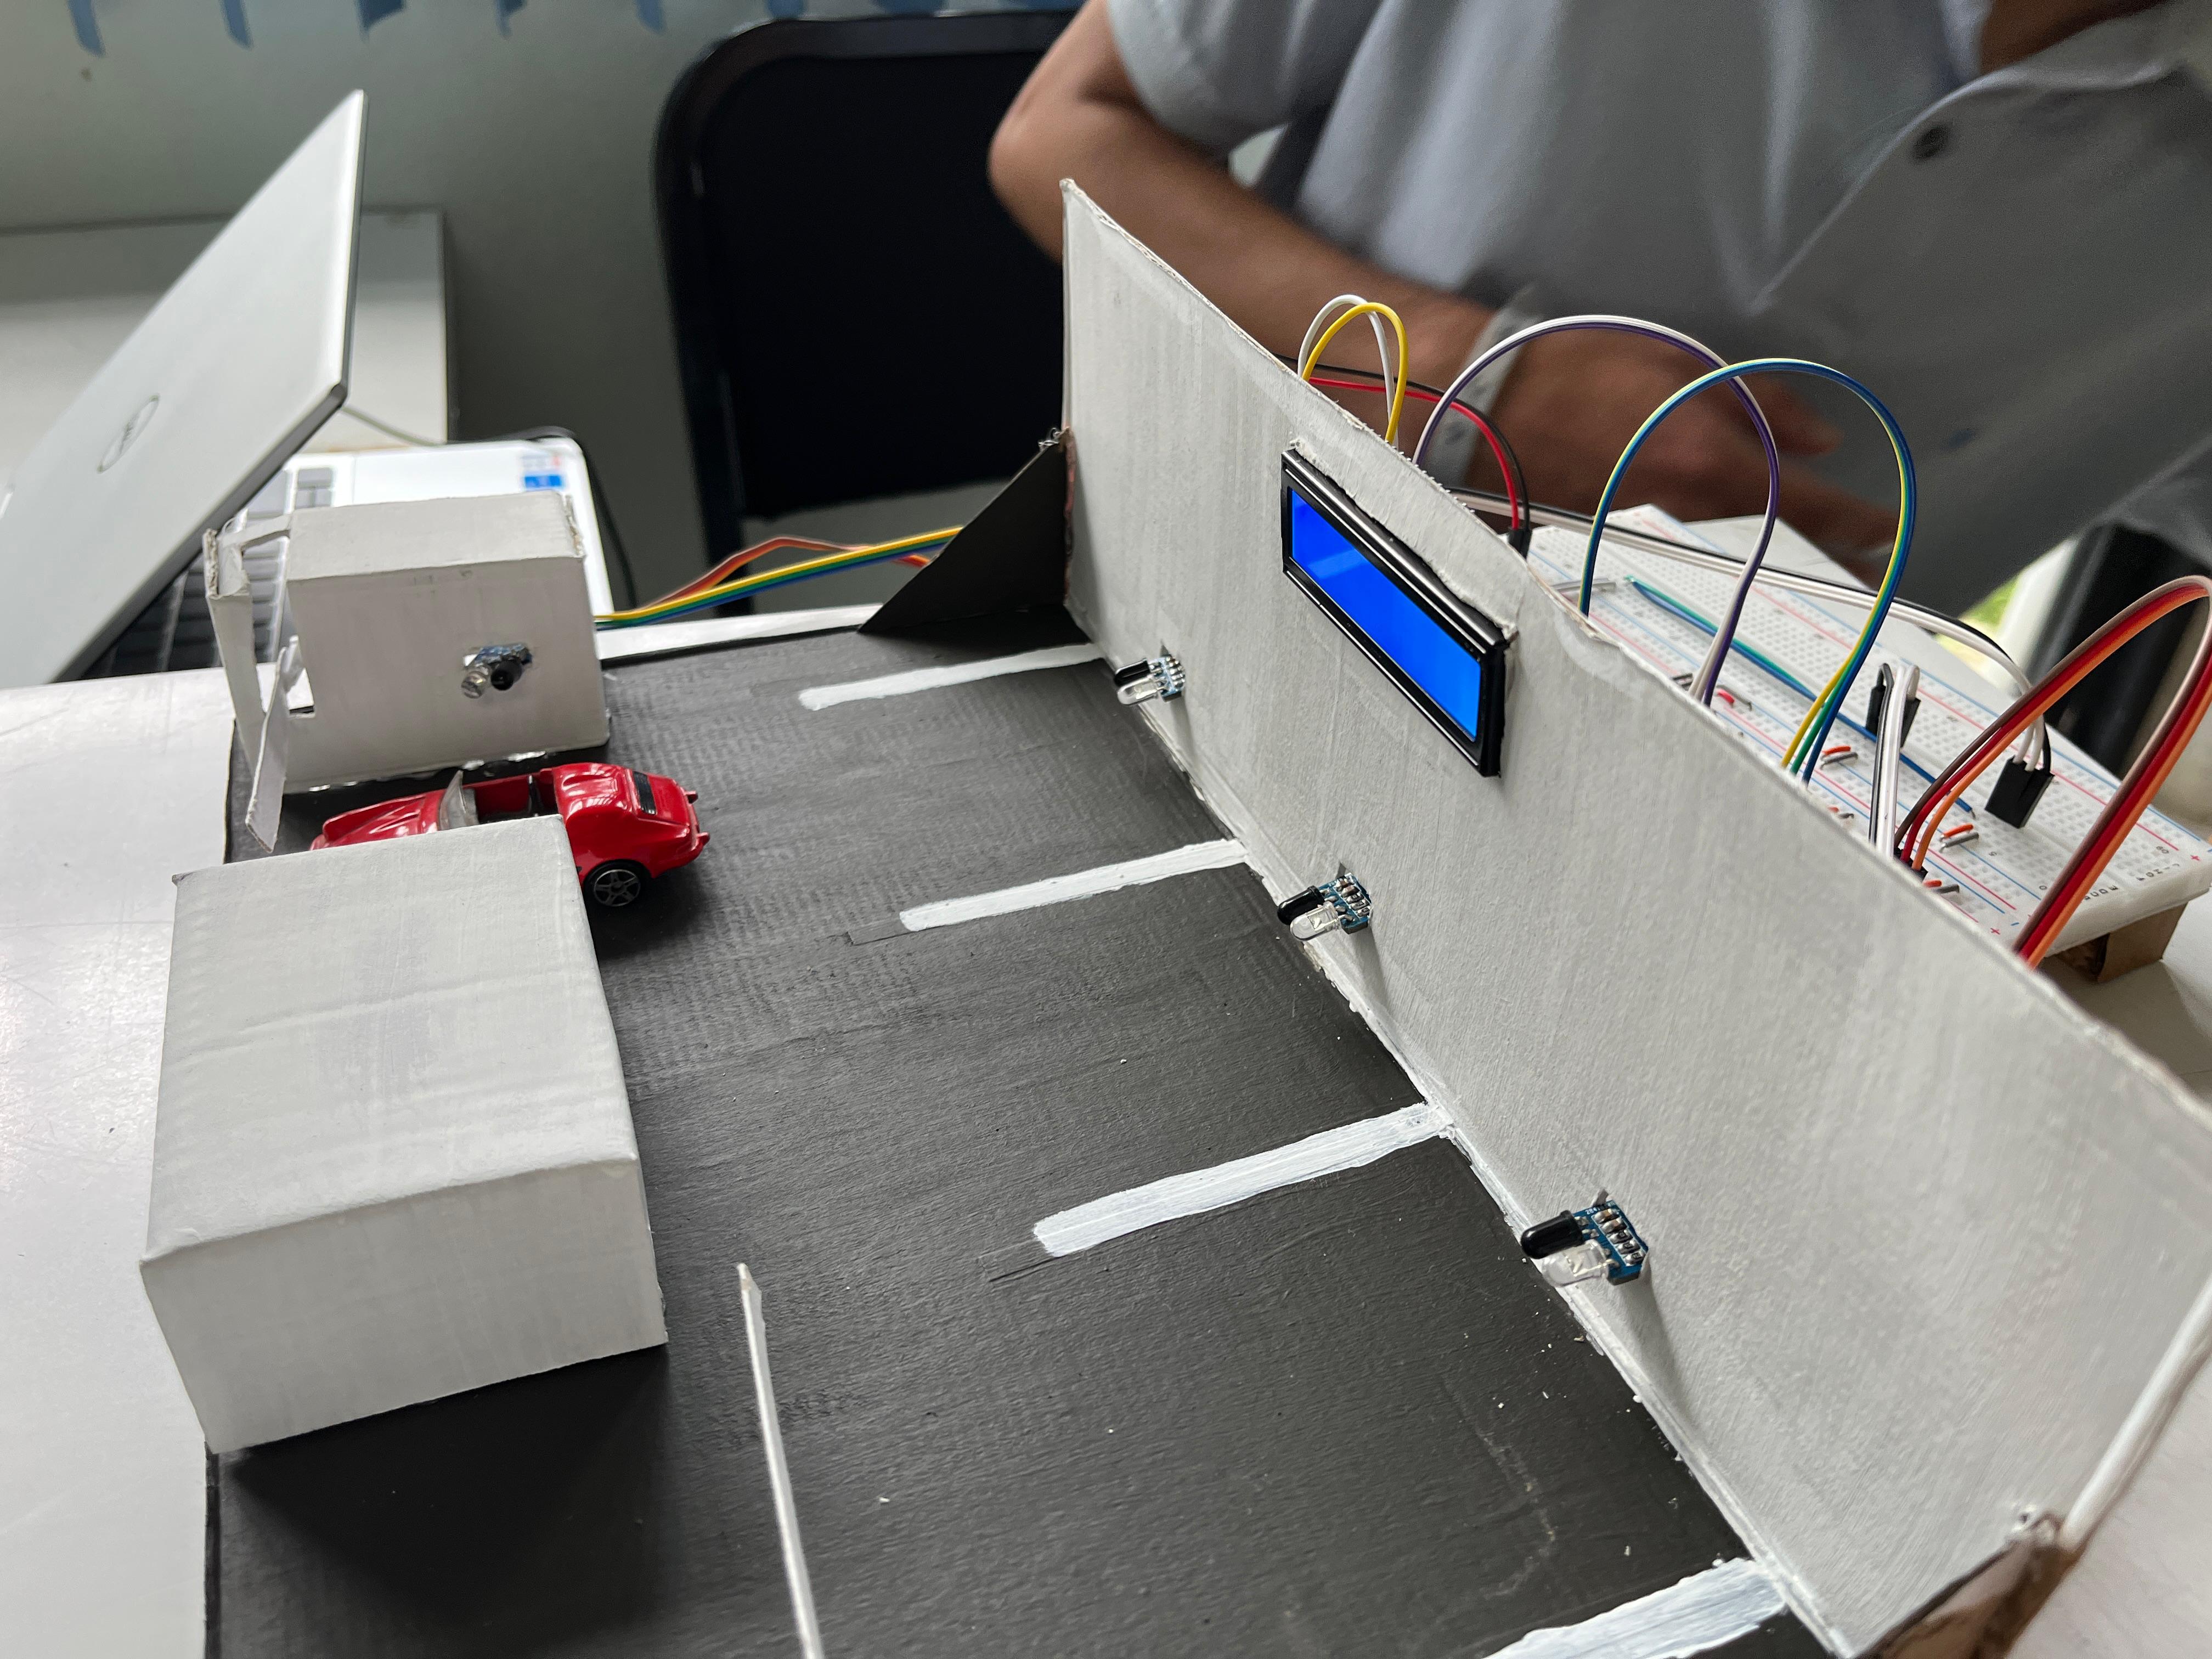
\includegraphics[width=0.8\linewidth]{Imagenes/inicial.jpeg}
    \caption{Maqueta del sistema de parqueo inteligente}
    \label{fig:100}
\end{figure}

\begin{figure}[H]
    \centering
    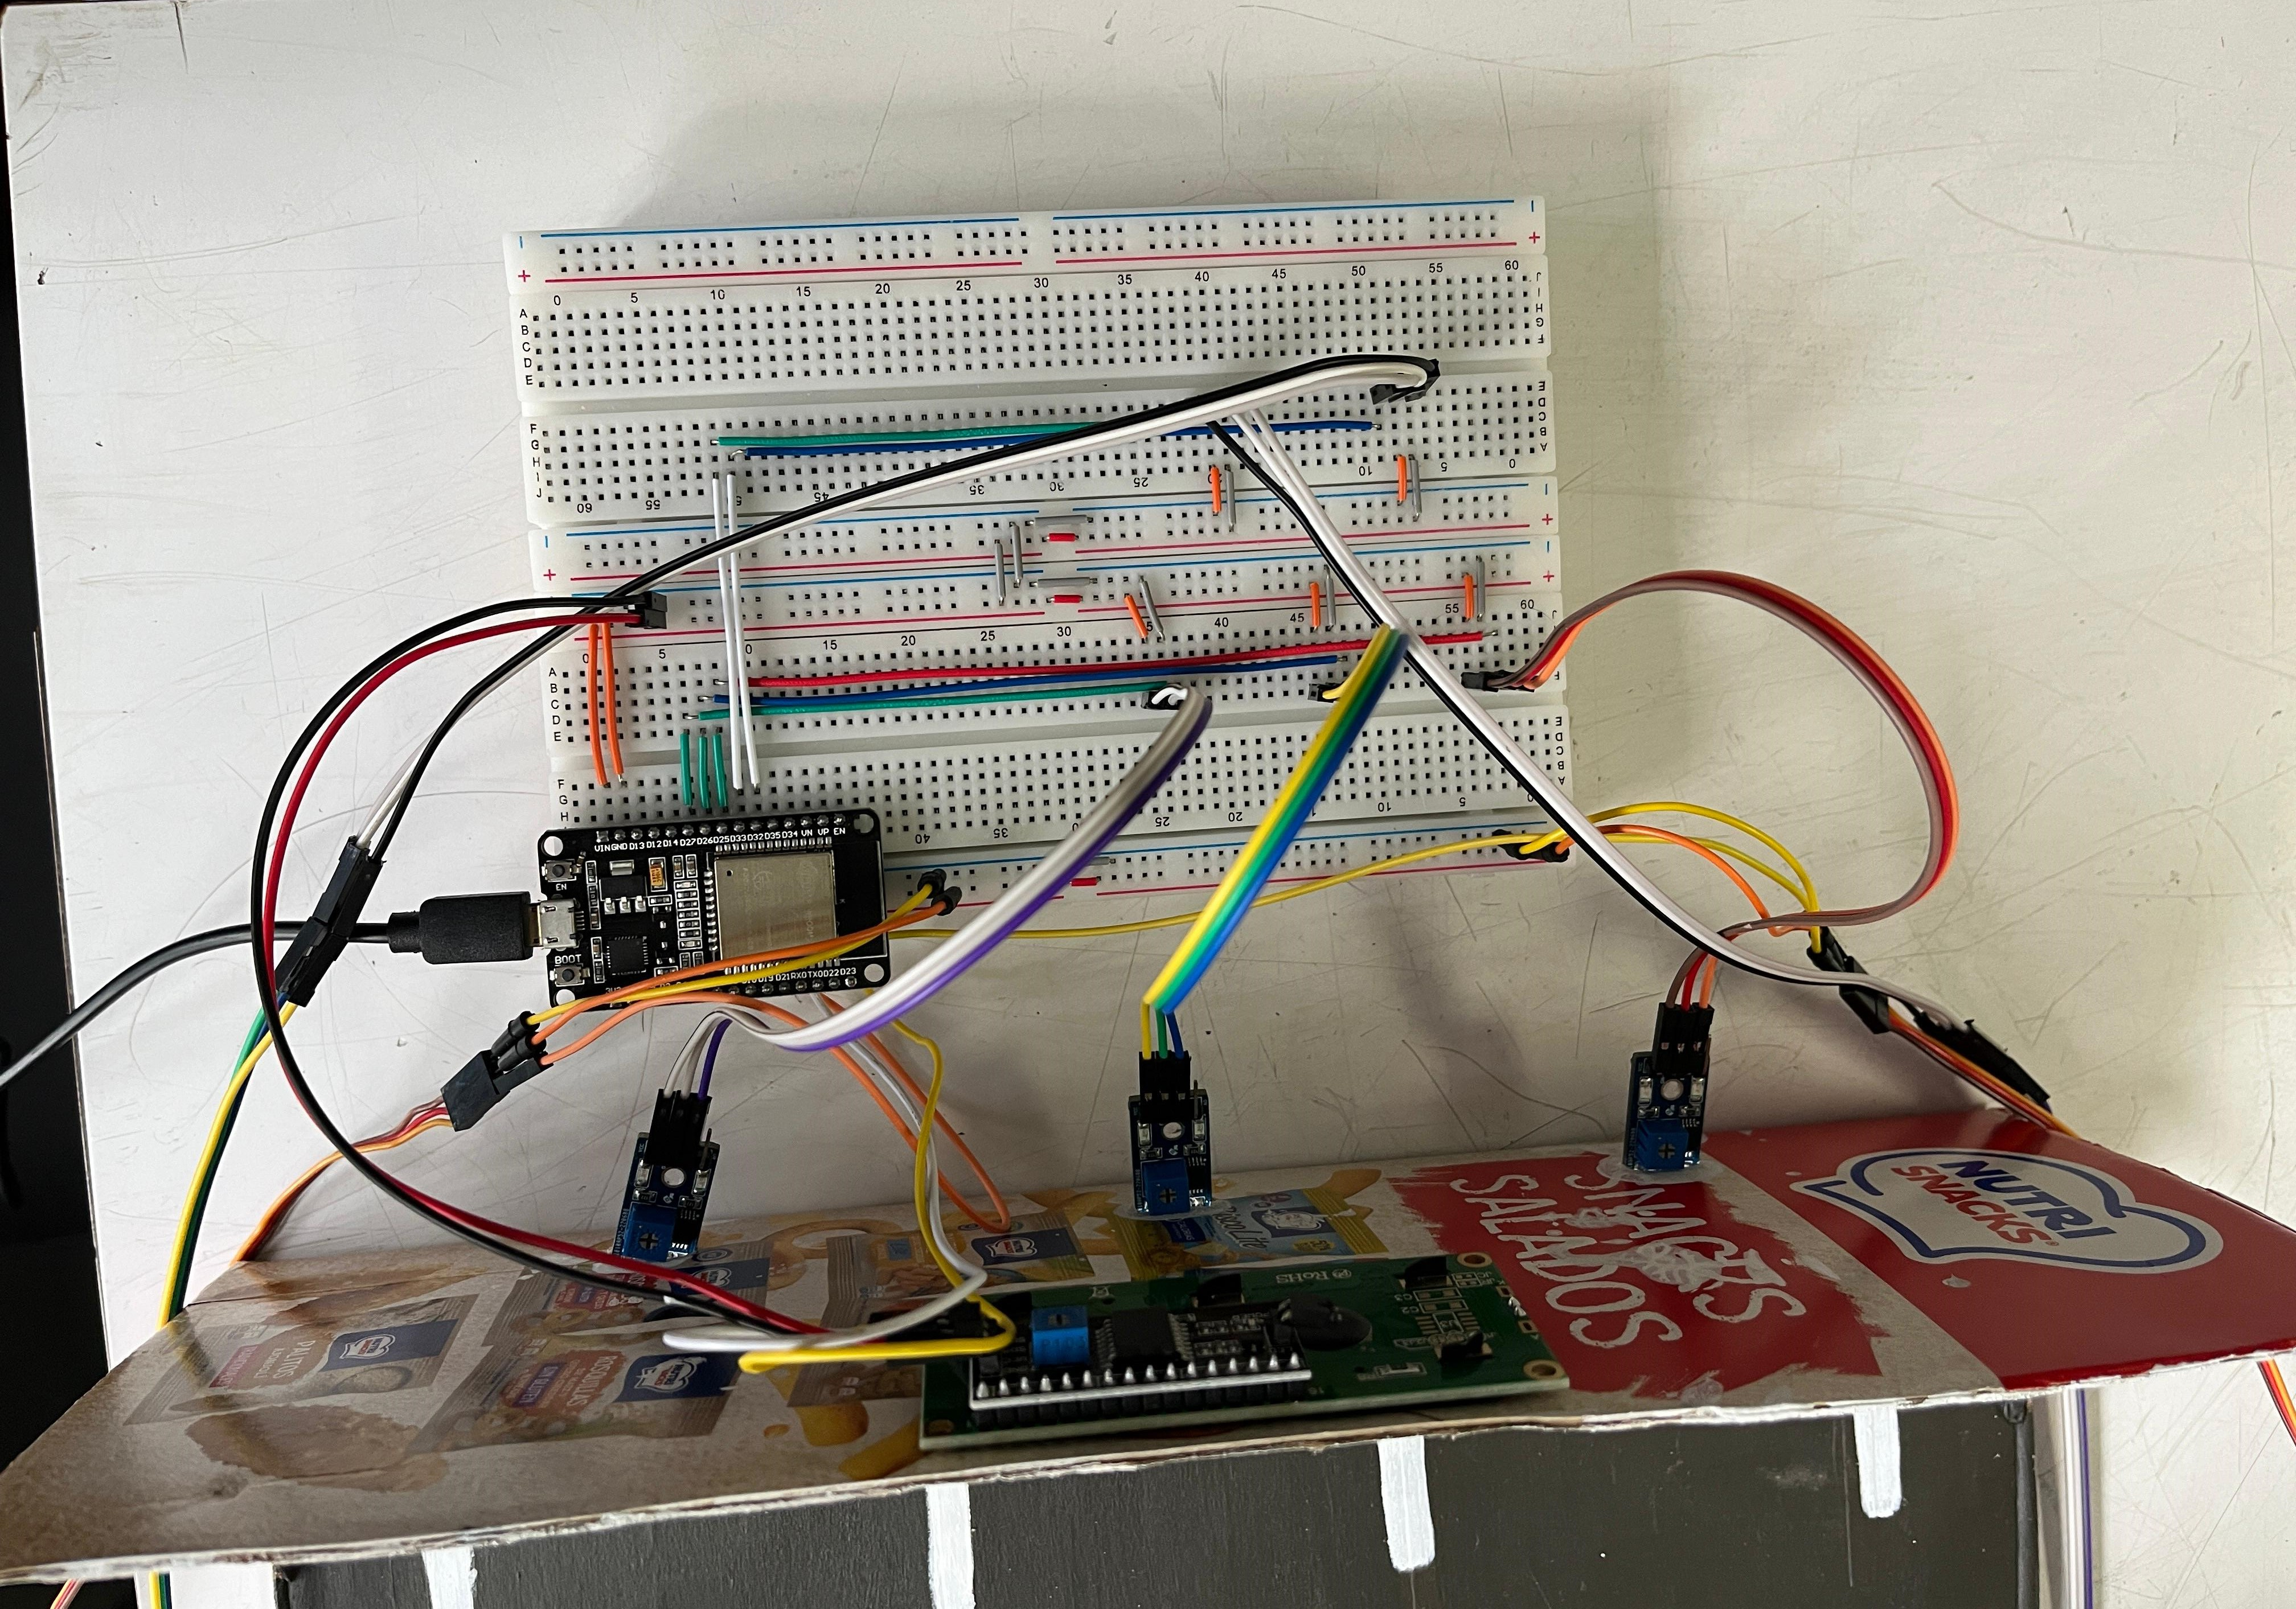
\includegraphics[width=0.8\linewidth]{Imagenes/circuito.jpeg}
    \caption{Circuito en protoboard del sistema}
    \label{fig:105}
\end{figure}

\subsection{Funcionamiento del Sistema}
El sistema opera de manera coordinada entre hardware y software para gestionar los espacios de parqueo de forma automatizada y remota. A continuación, se detalla su funcionamiento:

\subsubsection{Inicialización del Sistema}
El microcontrolador ESP32 se enciende y configura los periféricos:
    \begin{itemize}
        \item Los sensores infrarrojos se inicializan para detectar la presencia de vehículos y la entrada/salida.
        \item Los servomotores se posicionan en ``cerrado'' para las agujas.
        \item La pantalla LCD muestra el estado inicial de los espacios.
        \item Se establece la conexión Wi-Fi para comunicarse con la plataforma Blynk.
    \end{itemize}



\subsubsection{Gestión de Entrada de Vehículos}
\begin{enumerate}
    \item \textbf{Detección de entrada:}  
    El sensor infrarrojo en la entrada detecta la aproximación de un vehículo. El ESP32 envía una señal al servomotor de la entrada para que suba la aguja. 

    \item \textbf{Cierre de la aguja:}  
    Una vez que el vehículo pasa completamente, el sensor de entrada indica al servomotor que baje la aguja.
    
    \item \textbf{Actualización de disponibilidad:}  
    Los sensores en los espacios detectan la ocupación de un slot. El microcontrolador actualiza el estado a ``no disponible'' (\texttt{NA}) y reduce el contador total de espacios disponibles. Esta información se refleja en la pantalla LCD y en la aplicación móvil.
    

\end{enumerate}

\subsubsection{Gestión de Salida de Vehículos}
\begin{enumerate}
    \item \textbf{Liberación de espacio:}  
    Cuando el vehículo abandona un espacio, el sensor correspondiente detecta que está vacío. El sistema actualiza el estado del espacio a ``disponible'' (\texttt{A}) y aumenta el contador total de espacios disponibles.
    
    \item \textbf{Detección de salida:}  
    El sensor infrarrojo en la salida detecta el movimiento de un vehículo. El ESP32 envía una señal al servomotor de la salida para que suba la aguja.
    
    \item \textbf{Cierre de la aguja:}  
    El servomotor baja la aguja una vez que el vehículo ha salido por completo.
\end{enumerate}

\subsubsection{Visualización en la Pantalla LCD}
La pantalla LCD muestra en tiempo real el estado de los espacios de parqueo en el siguiente formato:
\begin{itemize}
    \item \texttt{Slot1:A, Slot2:A, Slot3:A, Total:3} (cuando todos los espacios están disponibles).
    \item \texttt{Slot1:NA, Slot2:A, Slot3:NA, Total:1} (si solo el segundo espacio está disponible, por ejemplo).
\end{itemize}
La información se actualiza dinámicamente cada vez que un sensor detecta un cambio en el estado.


\begin{figure}[H]
    \centering
    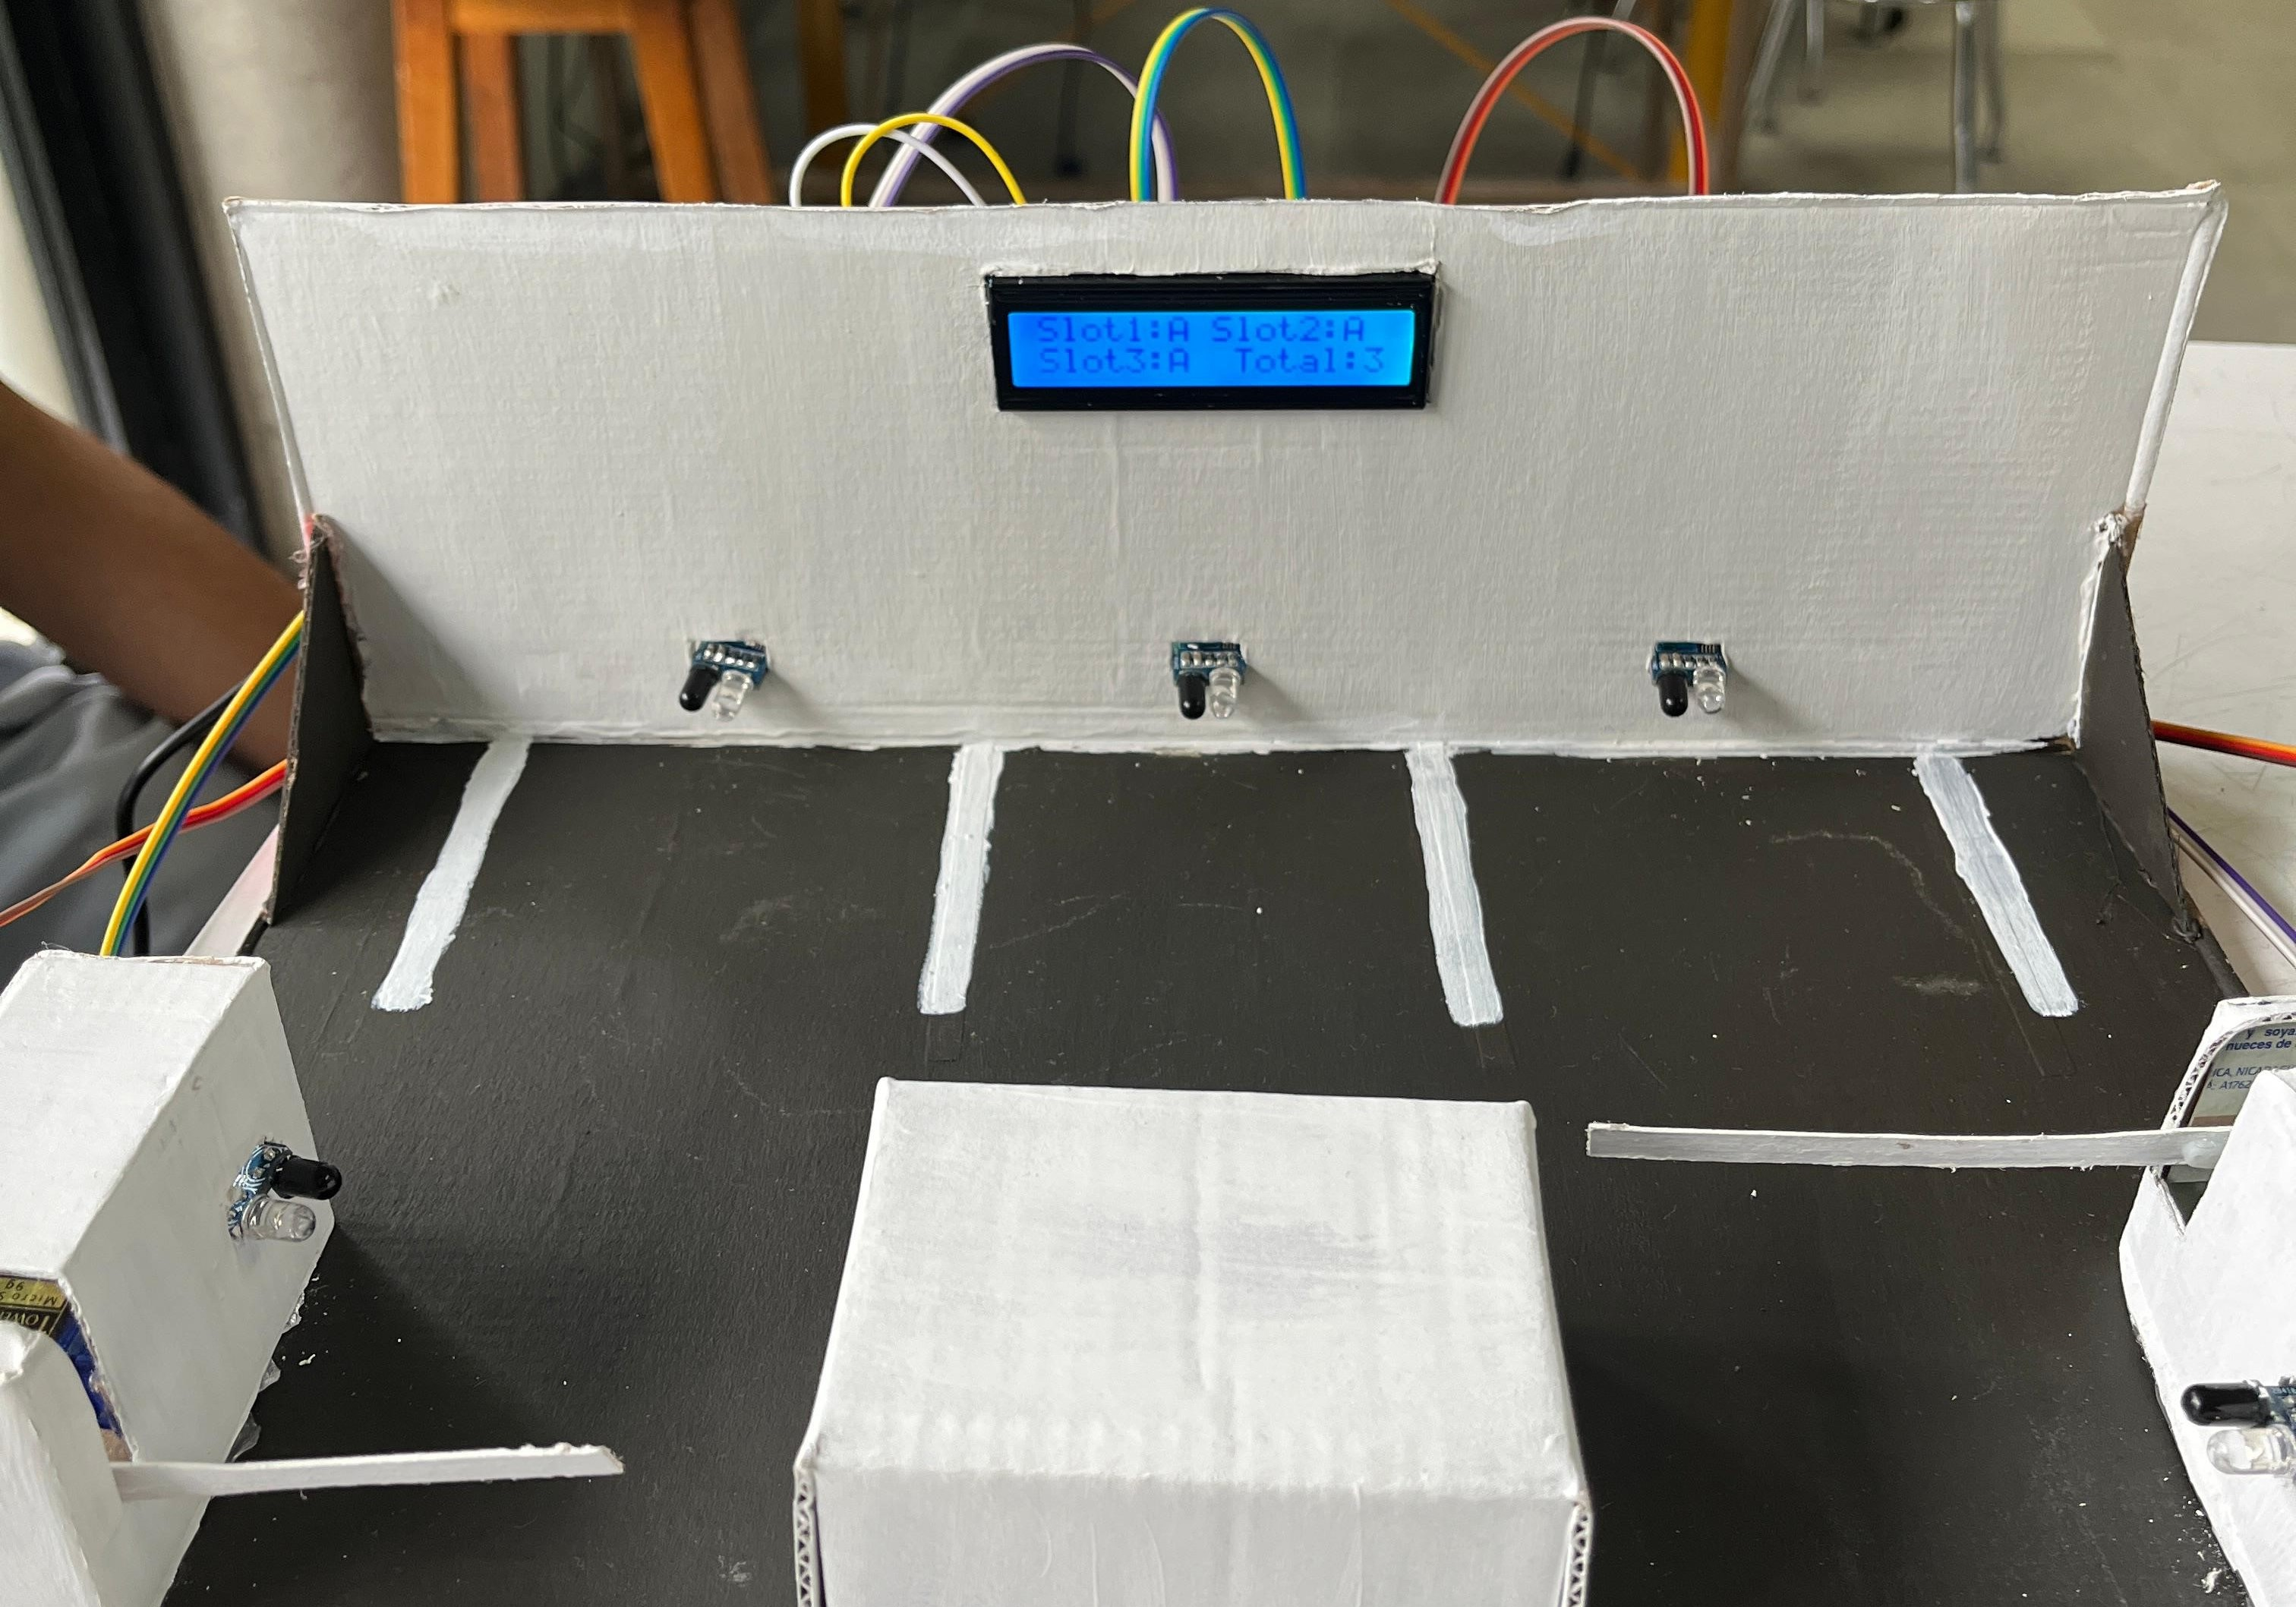
\includegraphics[width=0.8\linewidth]{Imagenes/lcd.jpeg}
    \caption{Visualización del estado de disponibilidad de los espacios en la pantalla LCD}
    \label{fig:101}
\end{figure}

\subsubsection{Control y Monitoreo Remoto con Blynk}
\begin{itemize}
    \item \textbf{Monitoreo:}  
    La aplicación móvil Blynk refleja el estado actual del parqueo, mostrando la disponibilidad de cada espacio (\texttt{0} para disponible, \texttt{1} para ocupado) y el total de espacios libres.

    \item \textbf{Reserva de espacios:}  
    La aplicación incluye un switch que permite a los usuarios reservar un espacio. Cuando se activa, el sistema marca el espacio como ``reservado'' incluso si está vacío.
\end{itemize}

\begin{figure}[H]
    \centering
    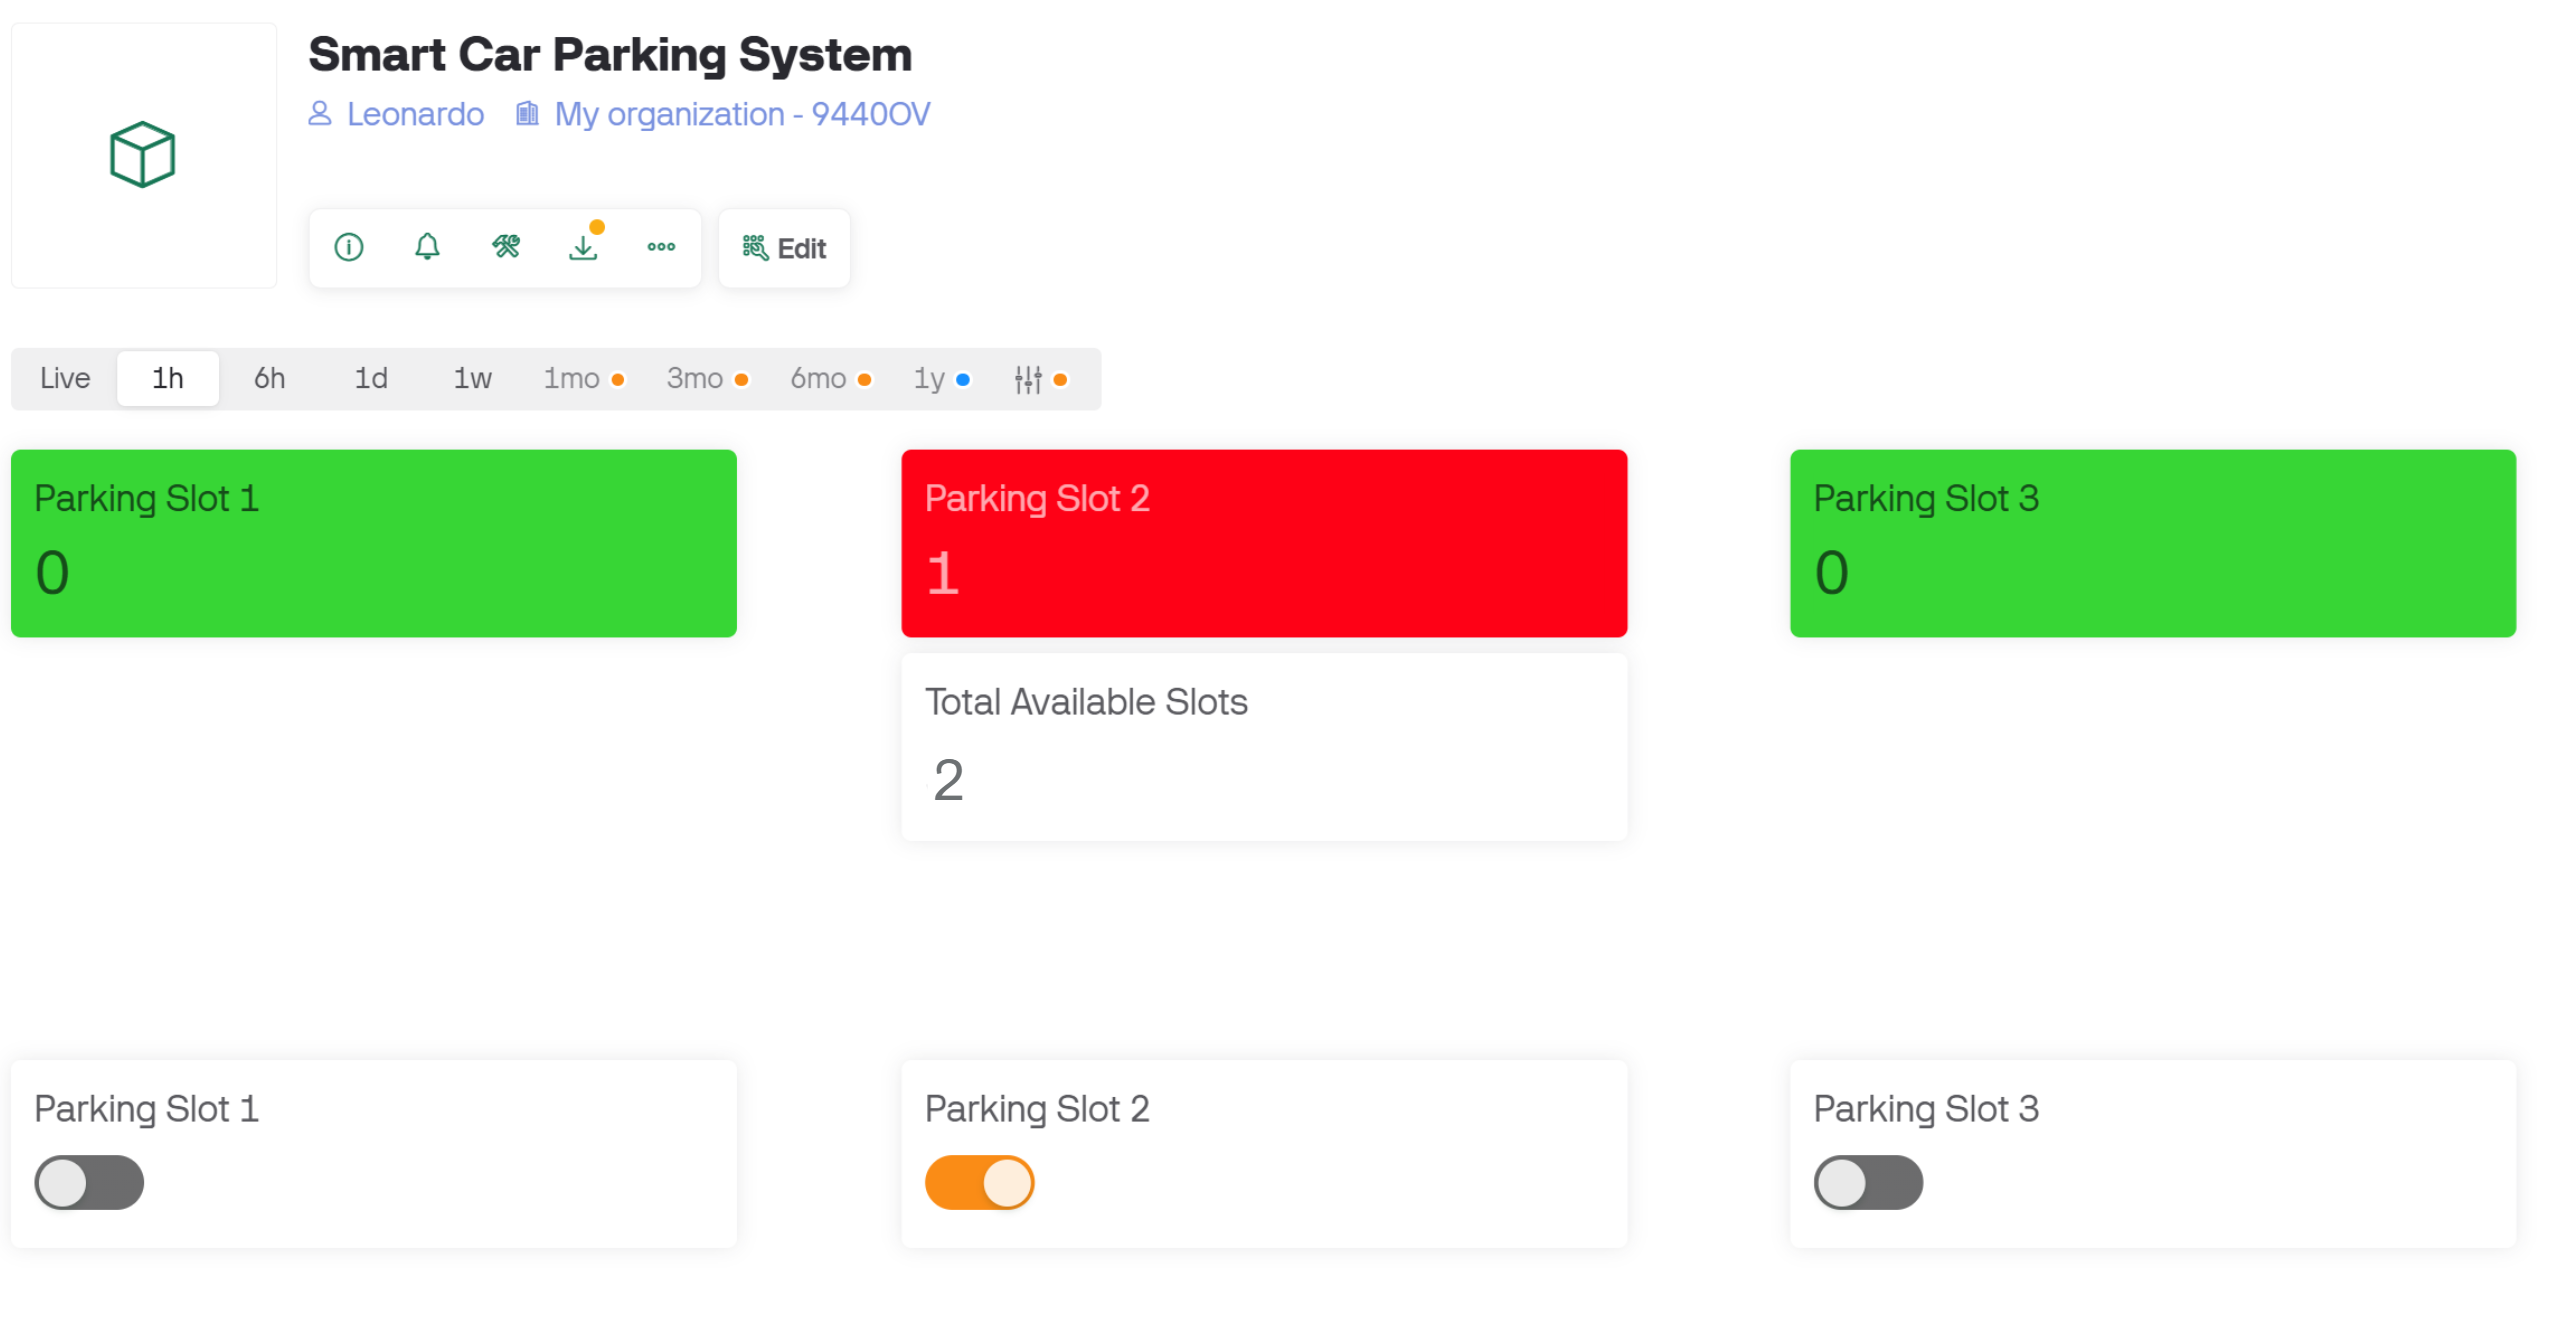
\includegraphics[width=1\linewidth]{Imagenes/blynk.png}
    \caption{Visualización de espacios disponibles en la plataforma Blynk por conexión WiFi cuando el slot 2 está ocupado}
    \label{fig:103}
\end{figure}



\subsection{Análisis de Resultados}
Los resultados obtenidos durante la implementación y pruebas del sistema de parqueo inteligente fueron satisfactorios, demostrando la efectividad de la integración entre los componentes de hardware y software. Los sensores infrarrojos presentaron un alto grado de precisión en la detección de vehículos en los espacios de parqueo y en las entradas/salidas, logrando una tasa de acierto sumamente alta. Sin embargo, se observó que en condiciones de iluminación ambiental intensa, la sensibilidad de los sensores disminuyó significativamente, lo que en algunos casos llevó a lecturas incorrectas. Este aspecto resalta la necesidad de considerar tecnologías complementarias para garantizar un desempeño consistente en diversas condiciones.

La sincronización entre el microcontrolador ESP32, la pantalla LCD y la plataforma Blynk se llevó a cabo de manera eficiente, permitiendo la actualización en tiempo real del estado de los espacios de parqueo tanto en la pantalla local como en la aplicación móvil. Los tiempos de respuesta en la aplicación fueron de aproximadamente 2 segundos, evidenciándose un retraso significativo en la actualización de datos en la plataforma Blynk. Por otro lado, la funcionalidad de reserva remota demostró ser útil y práctica.

En términos de automatización, el sistema logró operar sin intervención manual, controlando de manera precisa las agujas en las entradas y salidas mediante los servomotores, que respondieron rápidamente a las señales del ESP32. Esto significa una gran mejora en la experiencia del usuario al ingresar o salir del parqueo.

\section{Conclusiones y recomendaciones}

El sistema desarrollado cumplió con el objetivo de automatizar la detección y gestión de espacios de parqueo. La integración de sensores infrarrojos, servomotores y la pantalla LCD permitió un monitoreo local preciso, mientras que la conectividad con la plataforma Blynk ofreció una experiencia de usuario moderna y accesible. Esto demuestra que la implementación de tecnologías IoT puede optimizar significativamente la operación de estacionamientos, eliminando la necesidad de supervisión o accionamiento manual constante.

Se logró una integración con la aplicación Blynk que permite a los usuarios consultar la disponibilidad de espacios y realizar reservas en tiempo real desde cualquier lugar con conexión a Internet. Este aspecto no solo mejora la comodidad de los usuarios, sino que también evidencia la robustez del sistema en términos de comunicación y sincronización entre hardware y software.

Aunque el sistema funcionó correctamente, se identificaron algunas limitaciones, como la sensibilidad de los sensores infrarrojos a condiciones de luz ambiental extrema y los retrasos en la actualización de datos en la plataforma Blynk debido a las condiciones de la conexión Wi-Fi. Estas áreas representan oportunidades para mejorar la robustez y el desempeño general del sistema.

Para superar las limitaciones de los sensores infrarrojos, se recomienda explorar el uso de tecnologías complementarias como sensores ultrasónicos o cámaras con algoritmos de visión artificial. Estas herramientas pueden aumentar la precisión en la detección de vehículos, especialmente en condiciones de iluminación desfavorables.

Por otro lado, se recomienda optar por una pantalla LCD que ya cuente con el módulo I2C integrado, ya que adquirir ambos componentes por separado y soldar sus pines puede resultar más complejo, requiriendo de mayor tiempo y las herramientas adecuadas, además de aumentar el riesgo de errores durante el montaje, como conexiones inadecuadas o daños en los componentes.


\begin{thebibliography}{9}

\bibitem{iot}
AWS. (s.f.). ¿Qué es IoT (Internet de las cosas)?. Recuperado de \url{https://aws.amazon.com/es/what-is/iot/}

\bibitem{esp32}
Espressif Systems. (2019). ESP32 Series Datasheet (Version 3.0). Recuperado de \url{https://www.alldatasheet.com/datasheet-pdf/view/1148023/ESPRESSIF/ESP32.html}

\bibitem{sg90}
ETC. (s.f.). SG90 9g Micro Servo. Recuperado de \url{https://www.alldatasheet.es/datasheet-pdf/view/1572383/ETC/SG90.html}

\bibitem{irsensor}
Mactronica. (2024). Sensor de obstáculos infrarrojo. Recuperado de \url{https://www.mactronica.com.co/sensor-de-obstaculos-infrarrojo-fc-51}

\bibitem{fc51}
AG Electrónica SAPI de CV. (2024). Sensor de proximidad infrarrojo FC-51. Recuperado de \url{https://agelectronica.lat/pdfs/textos/O/OKY3127.PDF}

\bibitem{sfc51} UElectronics. (s.f.). FC-51 Sensor de Obstáculos Reflectivo Infrarrojo. Recuperado de  from https://uelectronics.com/producto/fc-51-sensor-de-obstaculos-reflectivo-infrarojo/


\bibitem{lcd}
SunFounder. (s.f.). I2C LCD 1602. Recuperado de \url{https://docs.sunfounder.com/projects/ultimate-sensor-kit/en/latest/components_basic/21-component_i2c_lcd1602.html}

\bibitem{lcd1602}
Handson Technology. (s.f.). I2C Serial Interface 1602 LCD Module. Recuperado de \url{https://www.handsontec.com/dataspecs/module/I2C_1602_LCD.pdf}


\bibitem{blynk} Blynk. (s.f.). Blynk: The platform for the Internet of Things. Recuperado de https://blynk.io/


\end{thebibliography}





\section{Anexos}

\includepdf[pages={8,12-16}]{Documentos/ESP32}
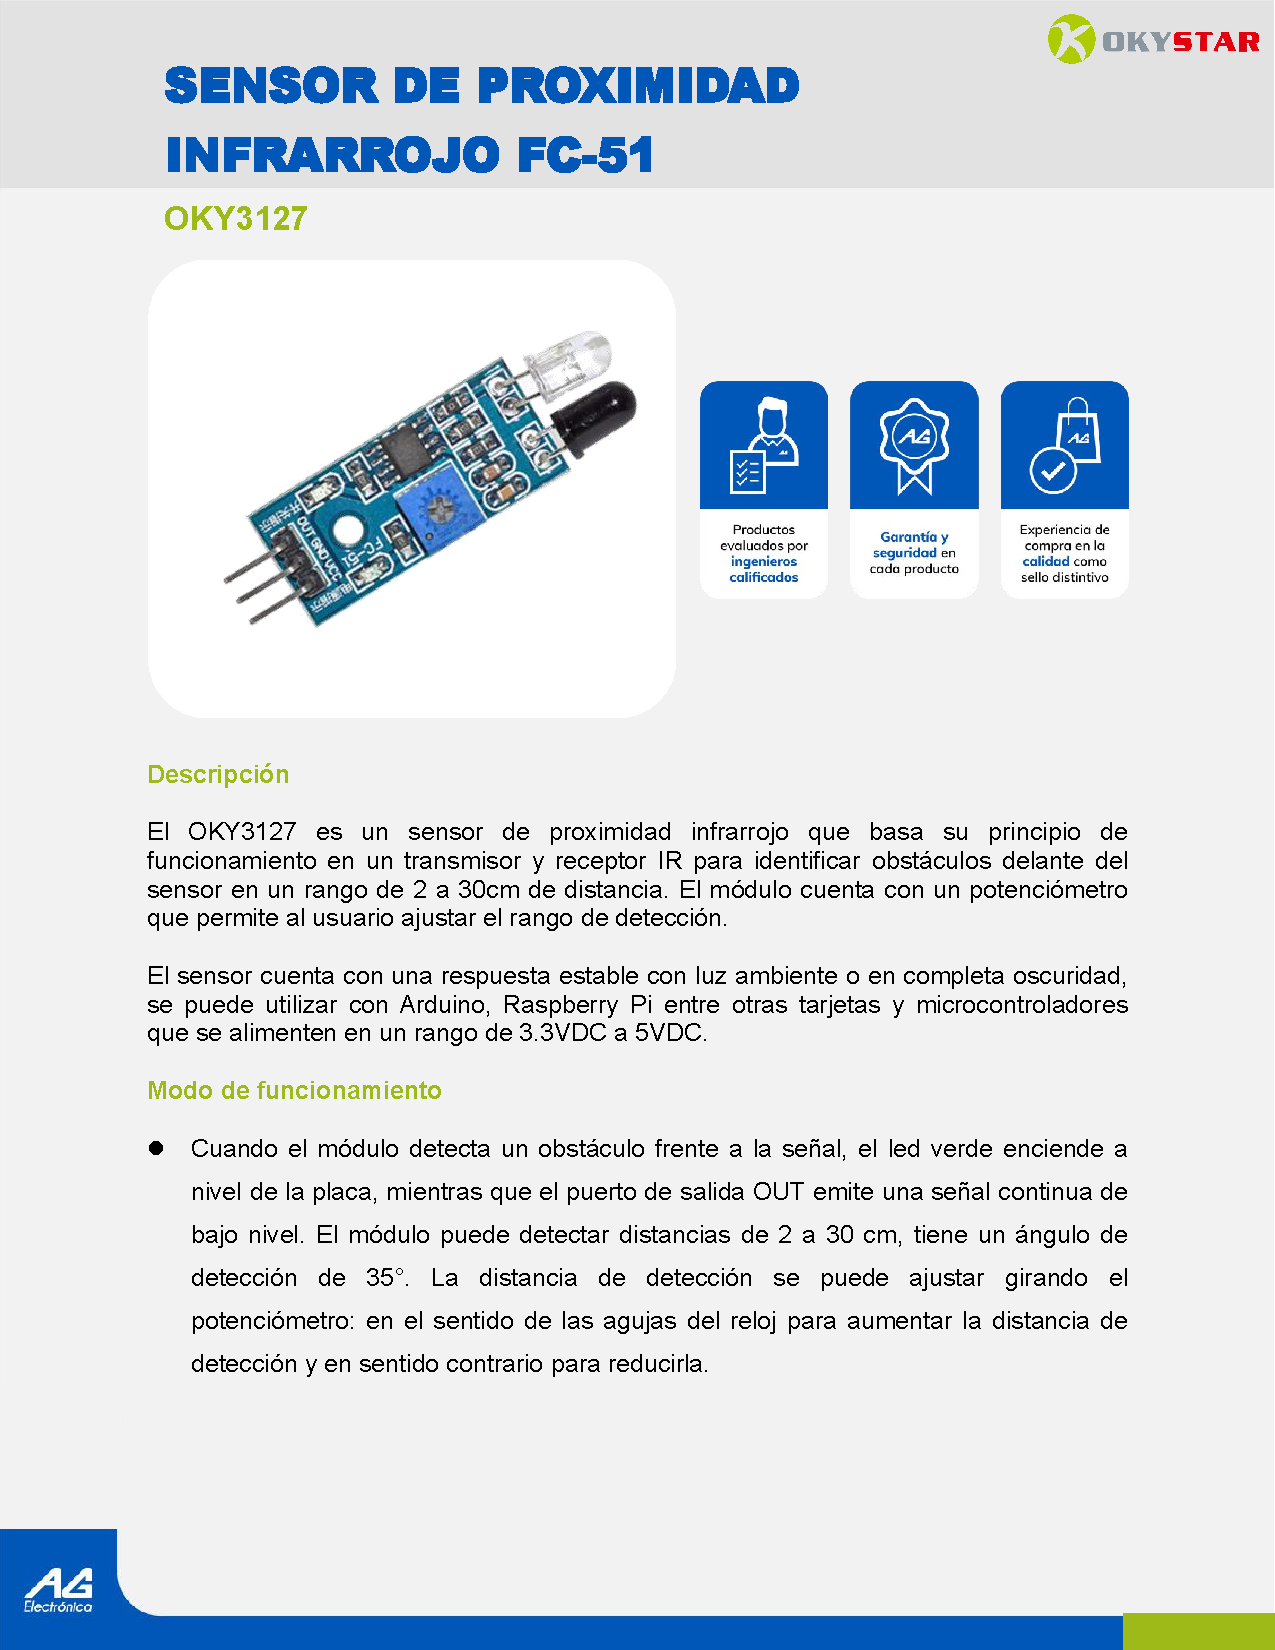
\includepdf[pages={1,2}]{Documentos/FC-51}
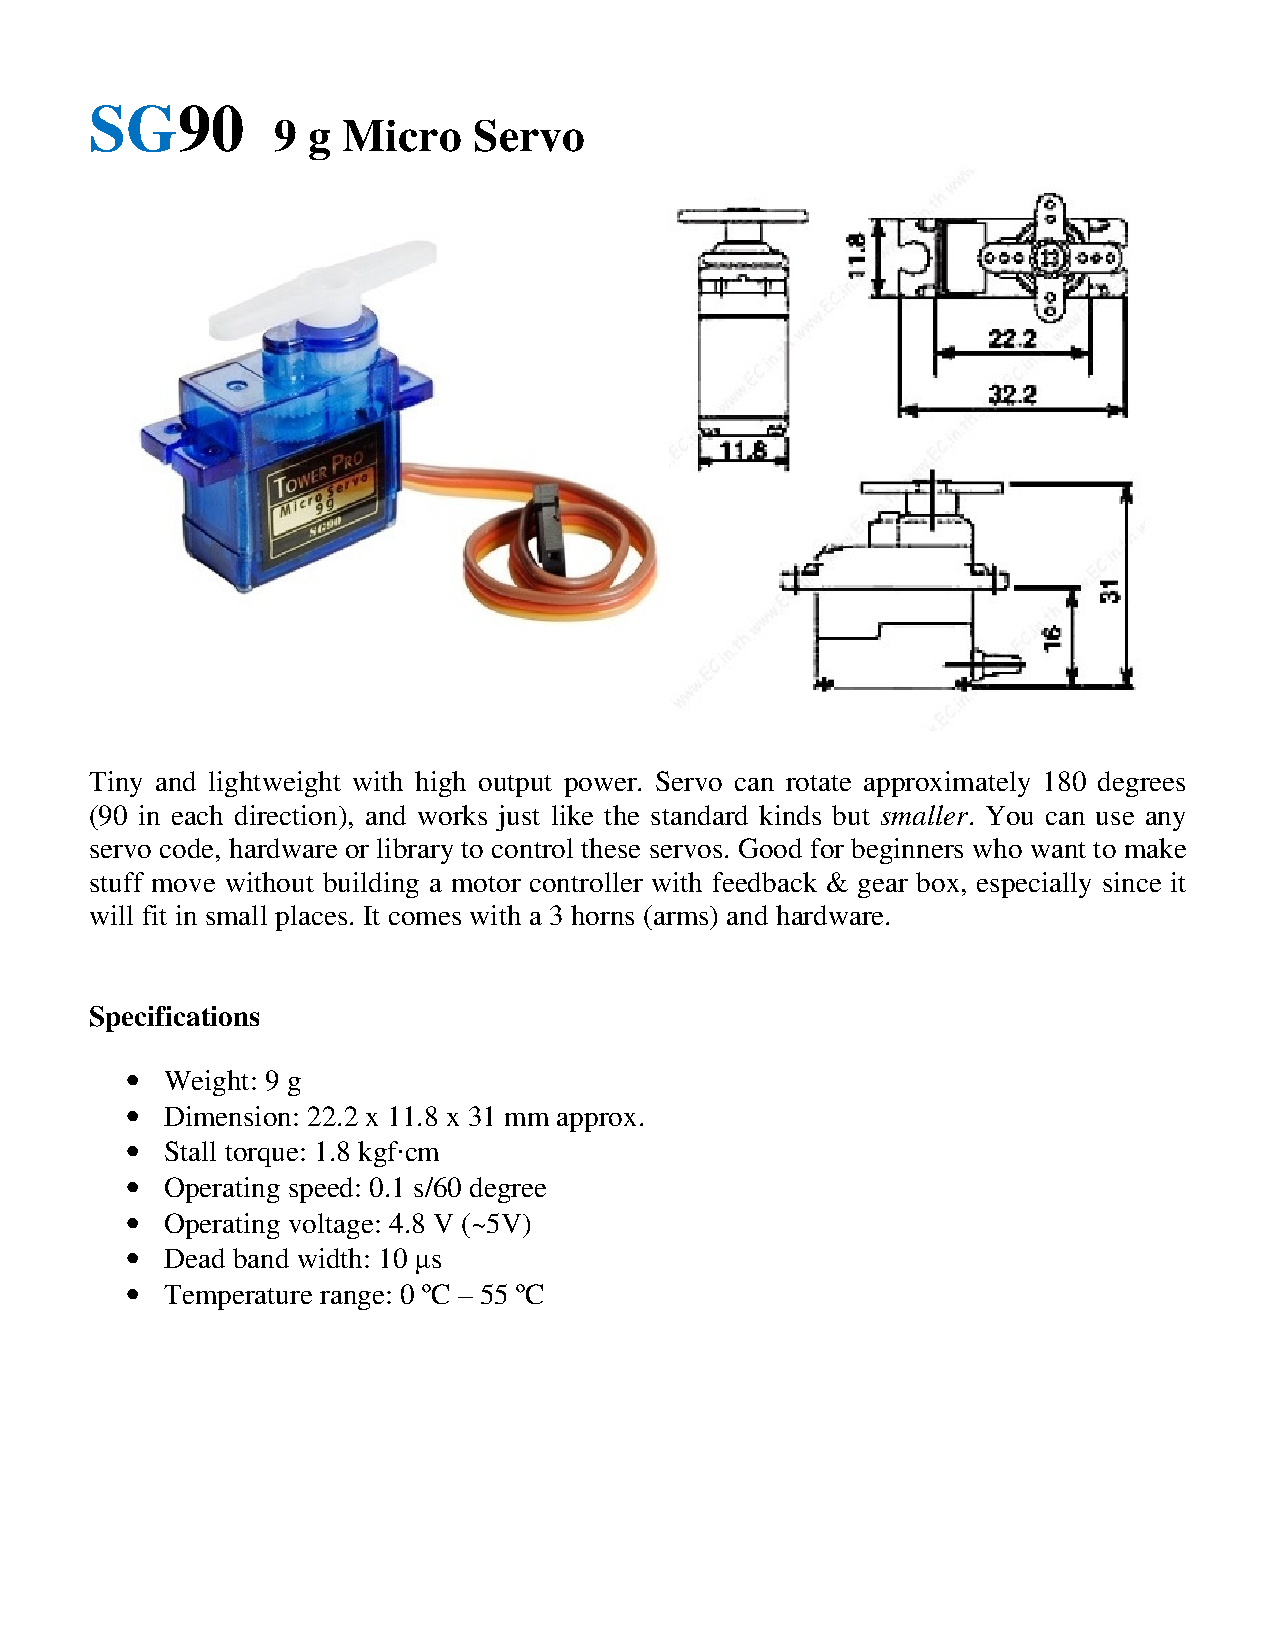
\includepdf[pages={1}]{Documentos/SG90}
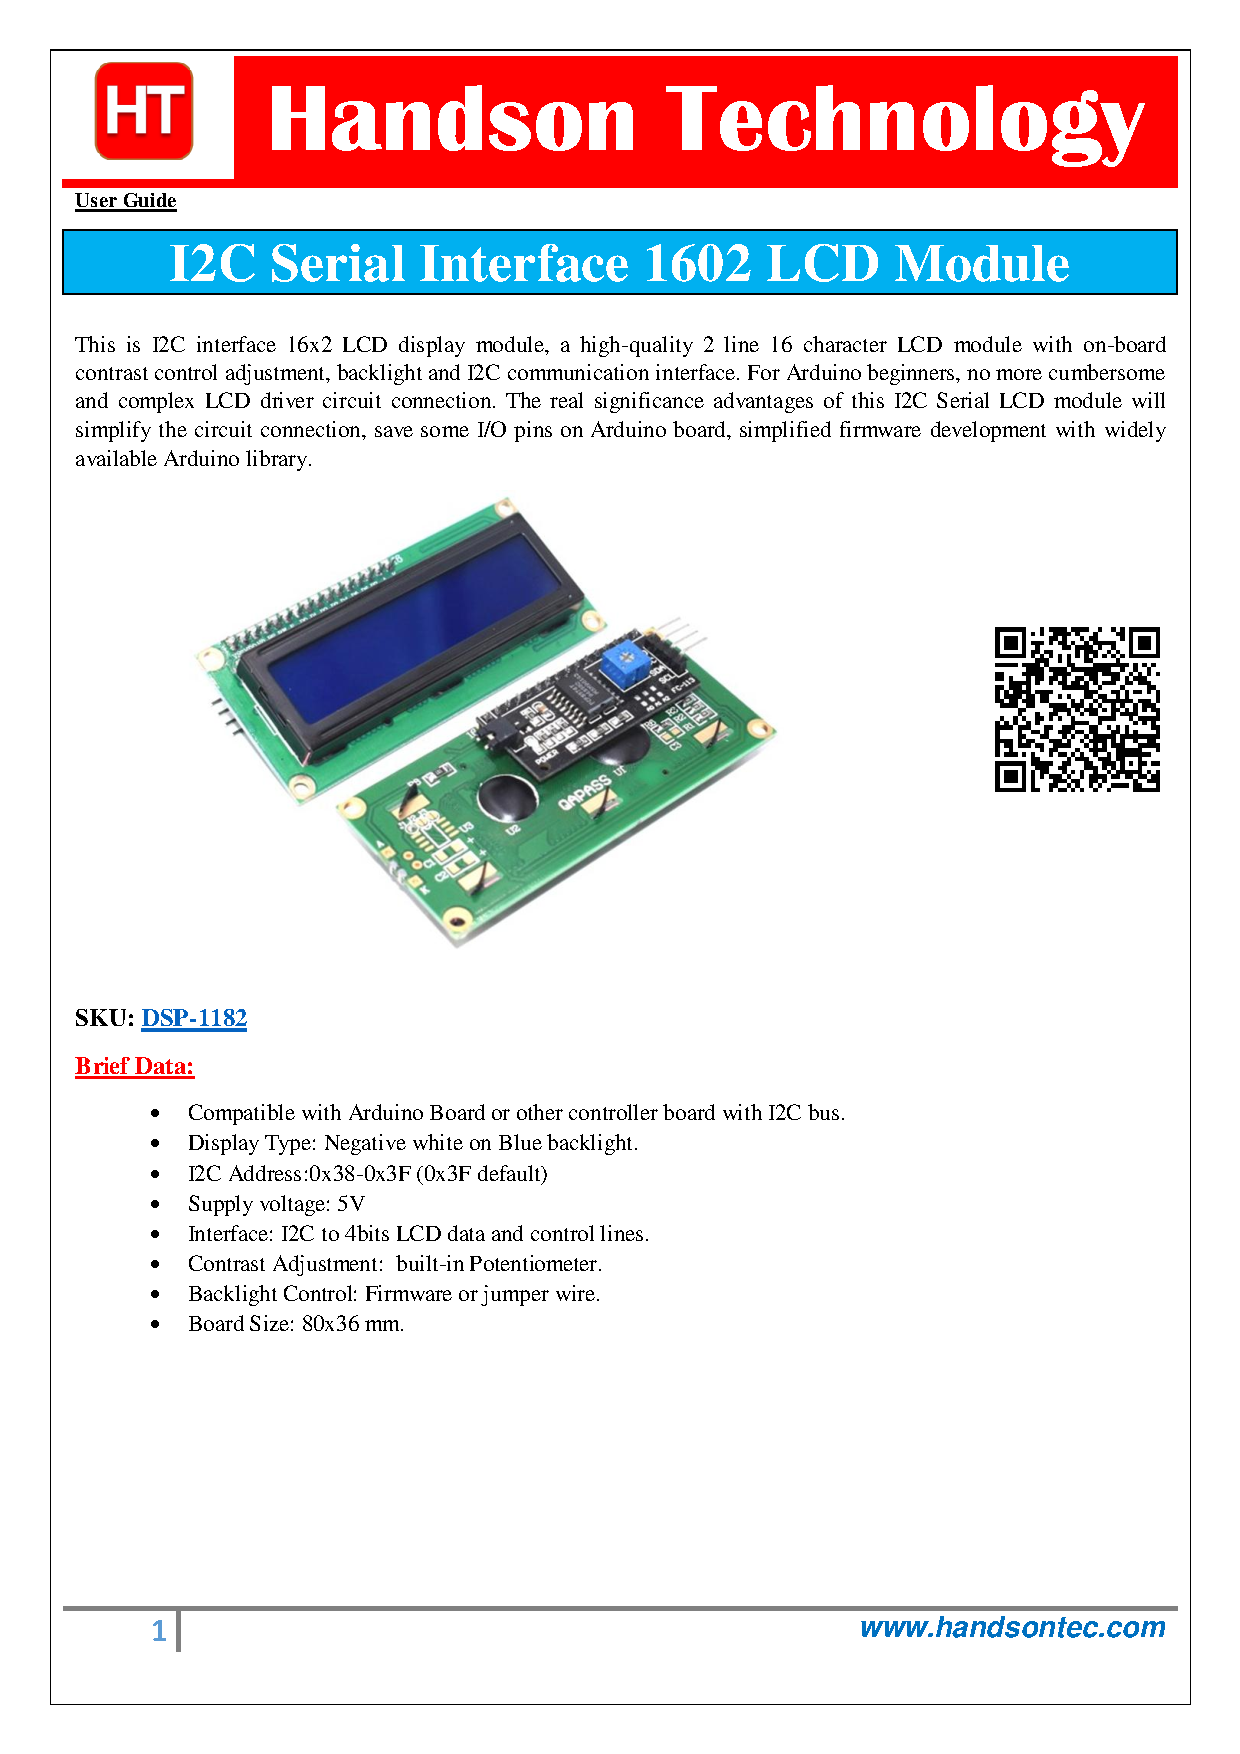
\includepdf[pages={1,2}]{Documentos/I2C_1602_LCD}



\end{document}
